\chapter{Advection-Diffusion QLBM}
\label{chapter:implementation}

\section{Algorithm}
\label{sec:algorithm}

My QLBM algorithm is heavily based on the work of Wawrzyniak et al. \cite{wawrzyniak2025base}, which in turn builds upon Budinski's original algorithm.
Their version extends the original algorithm to support nonuniform velocity fields and improves the initialization procedure.

Unlike all previous implementations I could find, I provide a truly generic, parameterized implementation that can work with any number of dimensions and any arbitrary set of links, including non-standard sets.
For the implementation I used the Qiskit framework and the Qiskit Aer Statevector simulator \cite{qiskit2024}.

An iteration of the algorithm consists of 4 steps:
\begin{enumerate}
    \item \textbf{Initialization}: Prepare the quantum state with the initial distribution function.
    \item \textbf{Collision}: Apply the collision operator to update the link distributions.
    \item \textbf{Streaming}: Propagate the link distributions to neighboring sites based on the link velocities.
    \item \textbf{Compute macros}: Recover the macroscopic distribution from the final state.
\end{enumerate}

Performing multiple iterations requires reinitializing the quantum state with the updated distribution function after each iteration.
If the velocity field or the link velocities change between iterations, the quantum circuit must be reconfigured accordingly.

Since the transpilation of the quantum circuit is the bottleneck of an iteration, instead of performing it each time, I transpile all \emph{distinct configurations} upfront and reuse the circuits during the simulation.
\section{Circuit Structure}
\label{sec:circuit}

\begin{figure}[H]
    \centering
    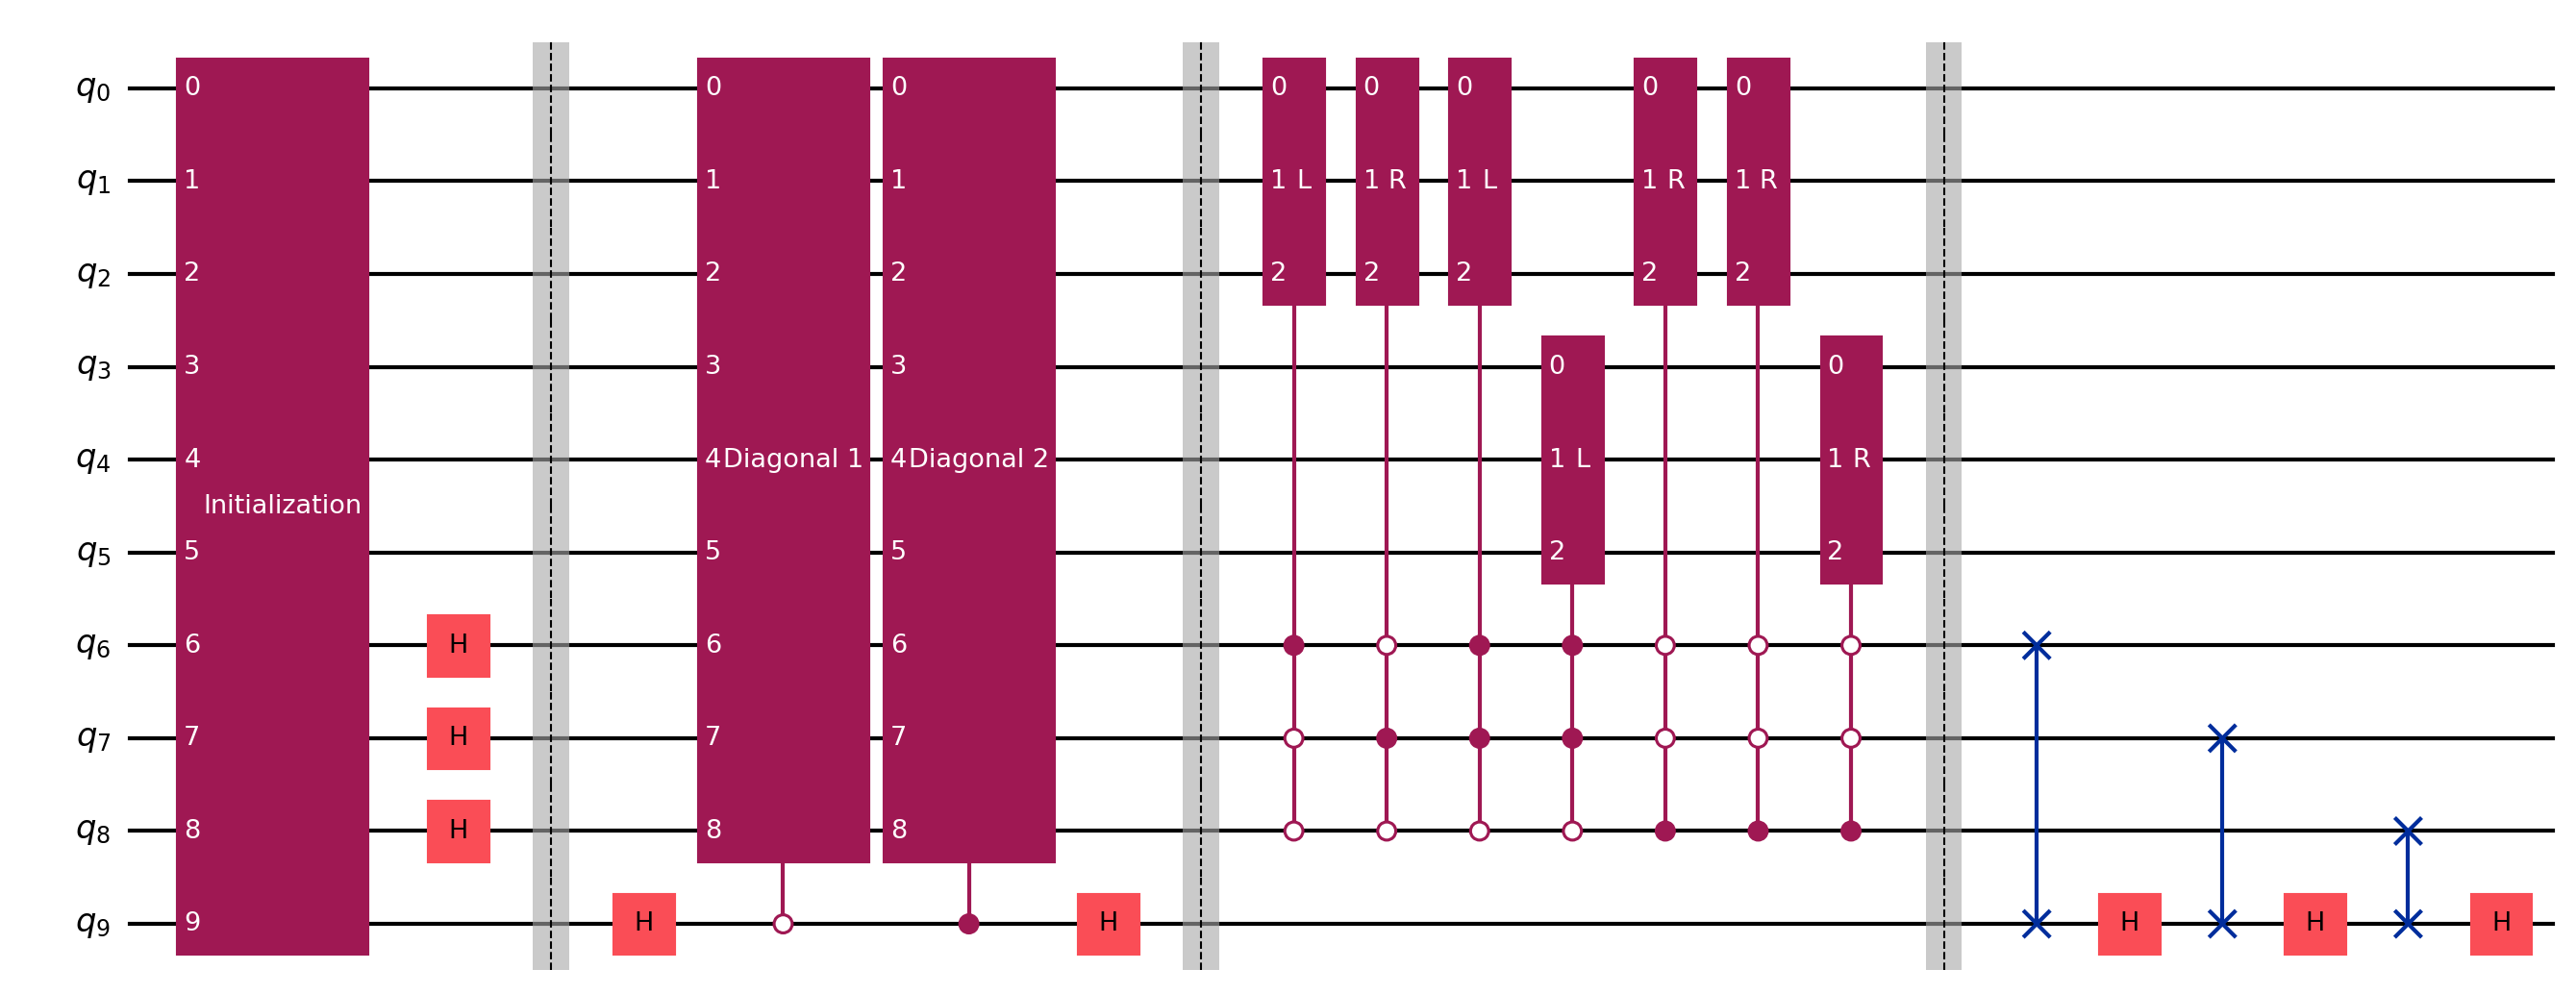
\includegraphics[width=\textwidth]{src/img/figures/complete_circuit.png}
    \caption{Complete quantum circuit for a single iteration of the QLBM algorithm. $q_{0-2}$ encode the X dimension, $q_{3-5}$ encode the Y dimension, $q_{6-8}$ encode the link velocities and $q_{9}$ is the ancilla qubit. The circuit is parameterized by the link velocities $[(0,0), (-1,0), (1,0), (-1,-1), (2,1)]$}
    \label{fig:complete_circuit}
\end{figure}

\paragraph*{Initialization}
The distribution function is flattened and encoded as amplitudes of a quantum state.
The number of qubits required for the total state is:
\begin{itemize}
    \item $n = \lceil \log_2(N) \rceil$, where $N$ is the number of links.
    \item $m = \sum_{i} \lceil \log_2(M_i) \rceil$, where $M_i$ is the number of lattice sites in dimension $i$.
    \item 1 ancilla qubit required for the Collision step.
\end{itemize}

The resulting state is:

\begin{equation}
    \ket{\psi} = \ket{0}\ket{0}^n\sum_{x} \frac{\Phi(x)}{||\Phi(x)||} \ket{x}
\end{equation}

Where the first qubit is the ancilla, the next $n$ qubits encode the link index and the remaining $m$ qubits encode the lattice site index.
The initialization is performed via Qiskit's \texttt{initialize} function to prepare a state given arbitrary amplitudes.

Following Wawrzyniak et al., I only initialize one of the link substates like this and make use of Hadamard gates to prepare the remaining substates.

\begin{equation}
    \ket{\psi} = \ket{0}\frac{1}{\sqrt{2^n}}\sum_{i}^{2^n} \ket{i}\sum_{x}\frac{\Phi(x)}{||\Phi(x)||} \ket{x}
\end{equation}

\paragraph*{Collision}
Starting from Equation~\ref{eq:bgk_operator} for the LBM BGK collision we can perform a common simplification by choosing $\tau=1$.
This implies that our distributions relax to the equilibrium each time step:
\begin{equation*}
    f_{i}^*(\mathbf{x}, t) = f_i^{\text{eq}}(\mathbf{x}, t)
\end{equation*}
This is standard for QLBM algorithms \cite{budinski2021quantum,wawrzyniak2025base} and follows a well known scheme in classical LBMs \cite{junk1999new}

From the Advection-Diffusion Equation (\ref{eq:advection-diffusion}), we can obtain a linear approximation and determine the formula for the equilibrium distribution:
\begin{equation}
    f_i^{eq} = w_i \Phi \left( 1 + \frac{\mathbf{c}_i \cdot \mathbf{u}(\mathbf{x},t)}{c_s^2} \right),
\end{equation}
with $w_i>0$ being the link weight, $c_i$ being the link velocity and $c_s$ a constant representing the speed of sound in the medium \cite{kruger2016lattice}.
In order to correctly approximate the ADE, these parameters must always obey:
\begin{align}
    \sum_{i} w_i &= 1 \\
    \sum_{i} w_i \mathbf{c}_{i\alpha} &= 0 \\
    \sum_{i} w_i \mathbf{c}_{i\alpha} \mathbf{c}_{i\beta} &= c_s^2 \delta_{\alpha\beta} \\
\end{align}

Since $\Phi$ is encoded in the amplitudes of the lattice qubits and the link qubits are in a uniform superposition, collision can be implemented as a single diagonal matrix $M$ of size $2^{m+n} \times 2^{m+n}$, where $m$ is the number of lattice qubits and $n$ is the number of link qubits.
\begin{equation*}
    M = \begin{pmatrix} 
    w_0 \left( 1 + \frac{\mathbf{c}_0 \cdot \mathbf{u}(\mathbf{x}_0,t)}{c_s^2} \right) & 0 & \dots & 0 \\
    0 & w_0 \left( 1 + \frac{\mathbf{c}_0 \cdot \mathbf{u}(\mathbf{x}_1,t)}{c_s^2} \right) & \dots & 0 \\
    \vdots & \vdots & \ddots & \vdots \\
    0 & 0 & \dots & w_{Q-1} \left( 1 + \frac{\mathbf{c}_{Q-1} \cdot \mathbf{u}(\mathbf{x}_{N-1},t)}{c_s^2} \right) 
    \end{pmatrix}
\end{equation*}

Assuming the simulation parameters are chosen accordingly, this matrix will conserve the $L_1$ norm of the state, corresponding to the conservation of mass.
This however is not sufficient in a quantum circuit, as preserving the $L_2$ norm is the requirement for unitarity.

Fortunately it can still be implemented as a block encoding, by writing
$M$ as a linear combination of unitaries $\frac{1}{2}(U_0 + U_1)$ with $U_0 = M + i\sqrt{I - M^2}$ and $U_1 = M - i\sqrt{I - M^2}$ \cite{low2019hamiltonian}.
The fact that the collision operator is diagonal is essential for this construction. More details in Appendix~\ref{app:collision_lcu}

Generally speaking, if the parameters respect the necessary preconditions to recover the ADE, then $M$ will be contractive, making the LCU technique possible. 
I used Qiskit's \texttt{DiagonalGate} to implement these unitaries.


The LCU circuit is identical to the one in Figure~\ref{fig:lcu_circuit}, with the mention that because both coefficients are eqaul,
the $P$ Gate is simply the $H$ Gate.

\paragraph*{Streaming}
Streaming involves propagating the link distributions to neighboring sites based on the link velocities.
The basic operation is shifting the amplitudes of a quantum state left or right, denoted as $LGate$ and $RGate$ respectively.

\begin{figure}[H]
    \centering
    \subfloat[$LGate$ for 4 qubits\label{fig:l_gate}]{%
        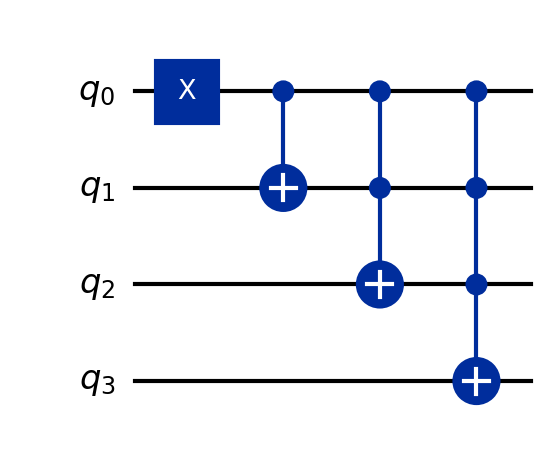
\includegraphics[width=0.45\textwidth]{src/img/figures/l_gate.png}%
    }
    \hfill
    \subfloat[$RGate$ for 4 qubits\label{fig:r_gate}]{%
        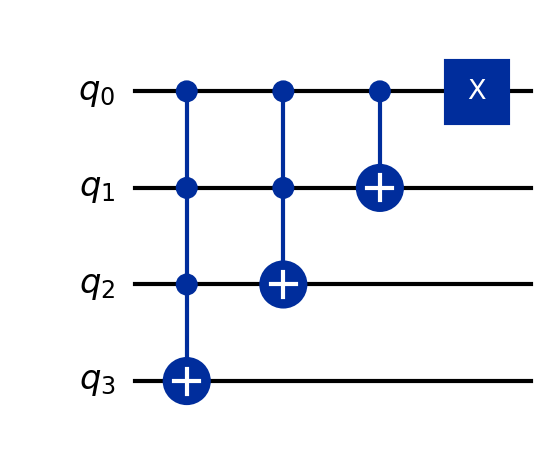
\includegraphics[width=0.45\textwidth]{src/img/figures/r_gate.png}%
    }
    \caption{Quantum circuits for implementing the streaming operation}
    \label{fig:streaming_gates}
\end{figure}

Conditionally applying these gates based on the binary encoding of the link index allows propagation of the link distributions for any arbitrary link velocity vector.
For example, to perform streaming by the velocity vector $(2,-1)$, one would apply the $RGate$ twice to the qubits encoding the first dimension and the $LGate$ once to the qubits encoding the second dimension.
These circuits "wrap" around upon reaching the boundary state, naturally implementing periodic boundary conditions.

\paragraph*{Computing Macroscopic Quantities}

Finally, the macroscopic distribution is recovered by summing over the link distributions.
This can be done both classically, after obtaining the final state or by applying a series of Hadamard and Swap gates to accumulate the distributions into a single link substate.

My implementation uses the quantum variant.
Lastly, the resultant distribution must be classically rescaled to the original norm because the quantum state was normalized.

\section{Experimental Validation}
\label{sec:validation}

To validate my implementation, I performed a series of experiments with various configurations and compared the results against classical simulations.
I could not find an existing classical simulator that would produce an output in a similar format, so I implemented a basic one.
The classical simulator follows the same collision formulas but avoids the pitfall of simply reimplementing the quantum algorithm as vector-matrix multiplication.
The speed of sound was the same in all experiments $c_s=\frac{1}{\sqrt{3}}$.

All code is open source and available at \url{https://github.com/widdrr/qlbm}

\paragraph*{1D Simulation}
\begin{itemize}
    \item \textbf{Configuration:} D1Q3 with 32 lattice sites for 50 iterations.
    \item \textbf{Links:} $\{(0),(-1),(1)\}$ with weights $\{2/3, 1/6, 1/6\}$.
    \item \textbf{Initial condition:} Gaussian hill centered at $x=8$, width $\sigma=2$ of amplitude $0.9$ and background $0.1$.
    \item \textbf{Velocity field:} Constant $u=0.3$ (rightward advection).
\end{itemize}

\begin{figure}[H]
    \centering
    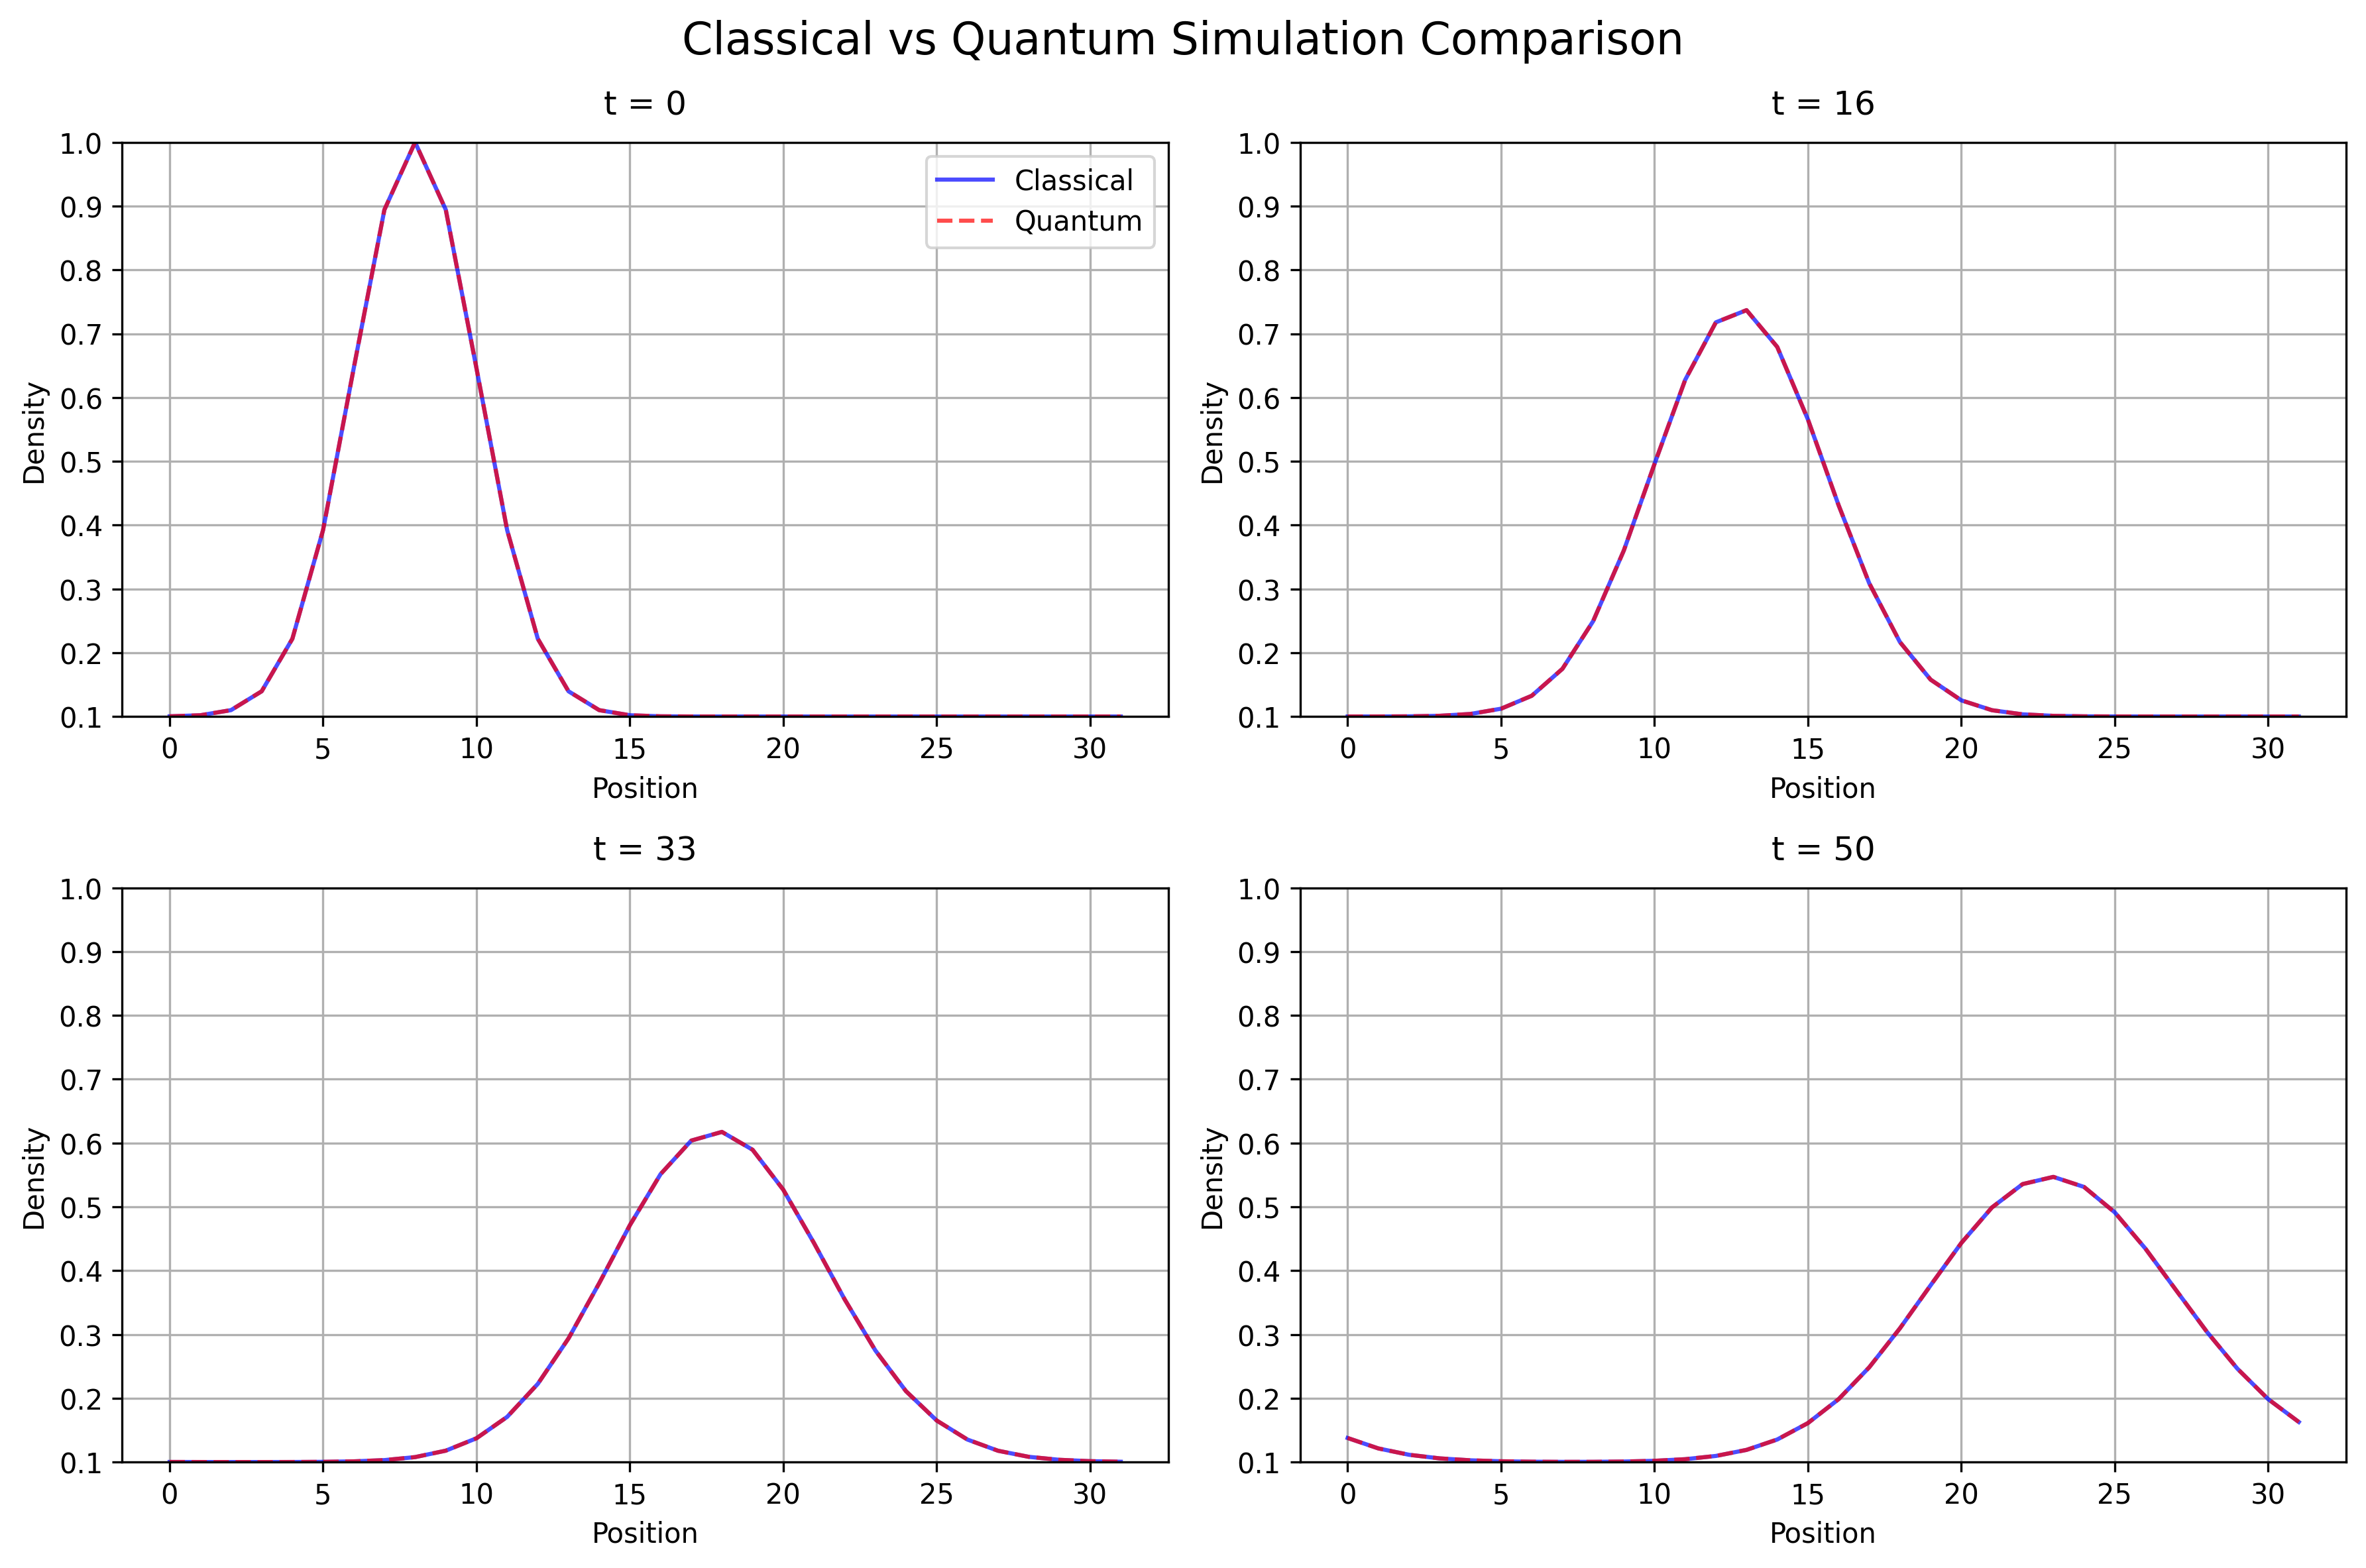
\includegraphics[width=0.8\textwidth]{src/img/figures/1_Dcomparison.png}
    \caption{Comparison of quantum and classical simulations for the 1D case}
    \label{fig:1d_comparison}
\end{figure}

The RMSE shows an exact match with the classical simulation, accounting for floating point errors.

\begin{figure}[H]
    \centering
    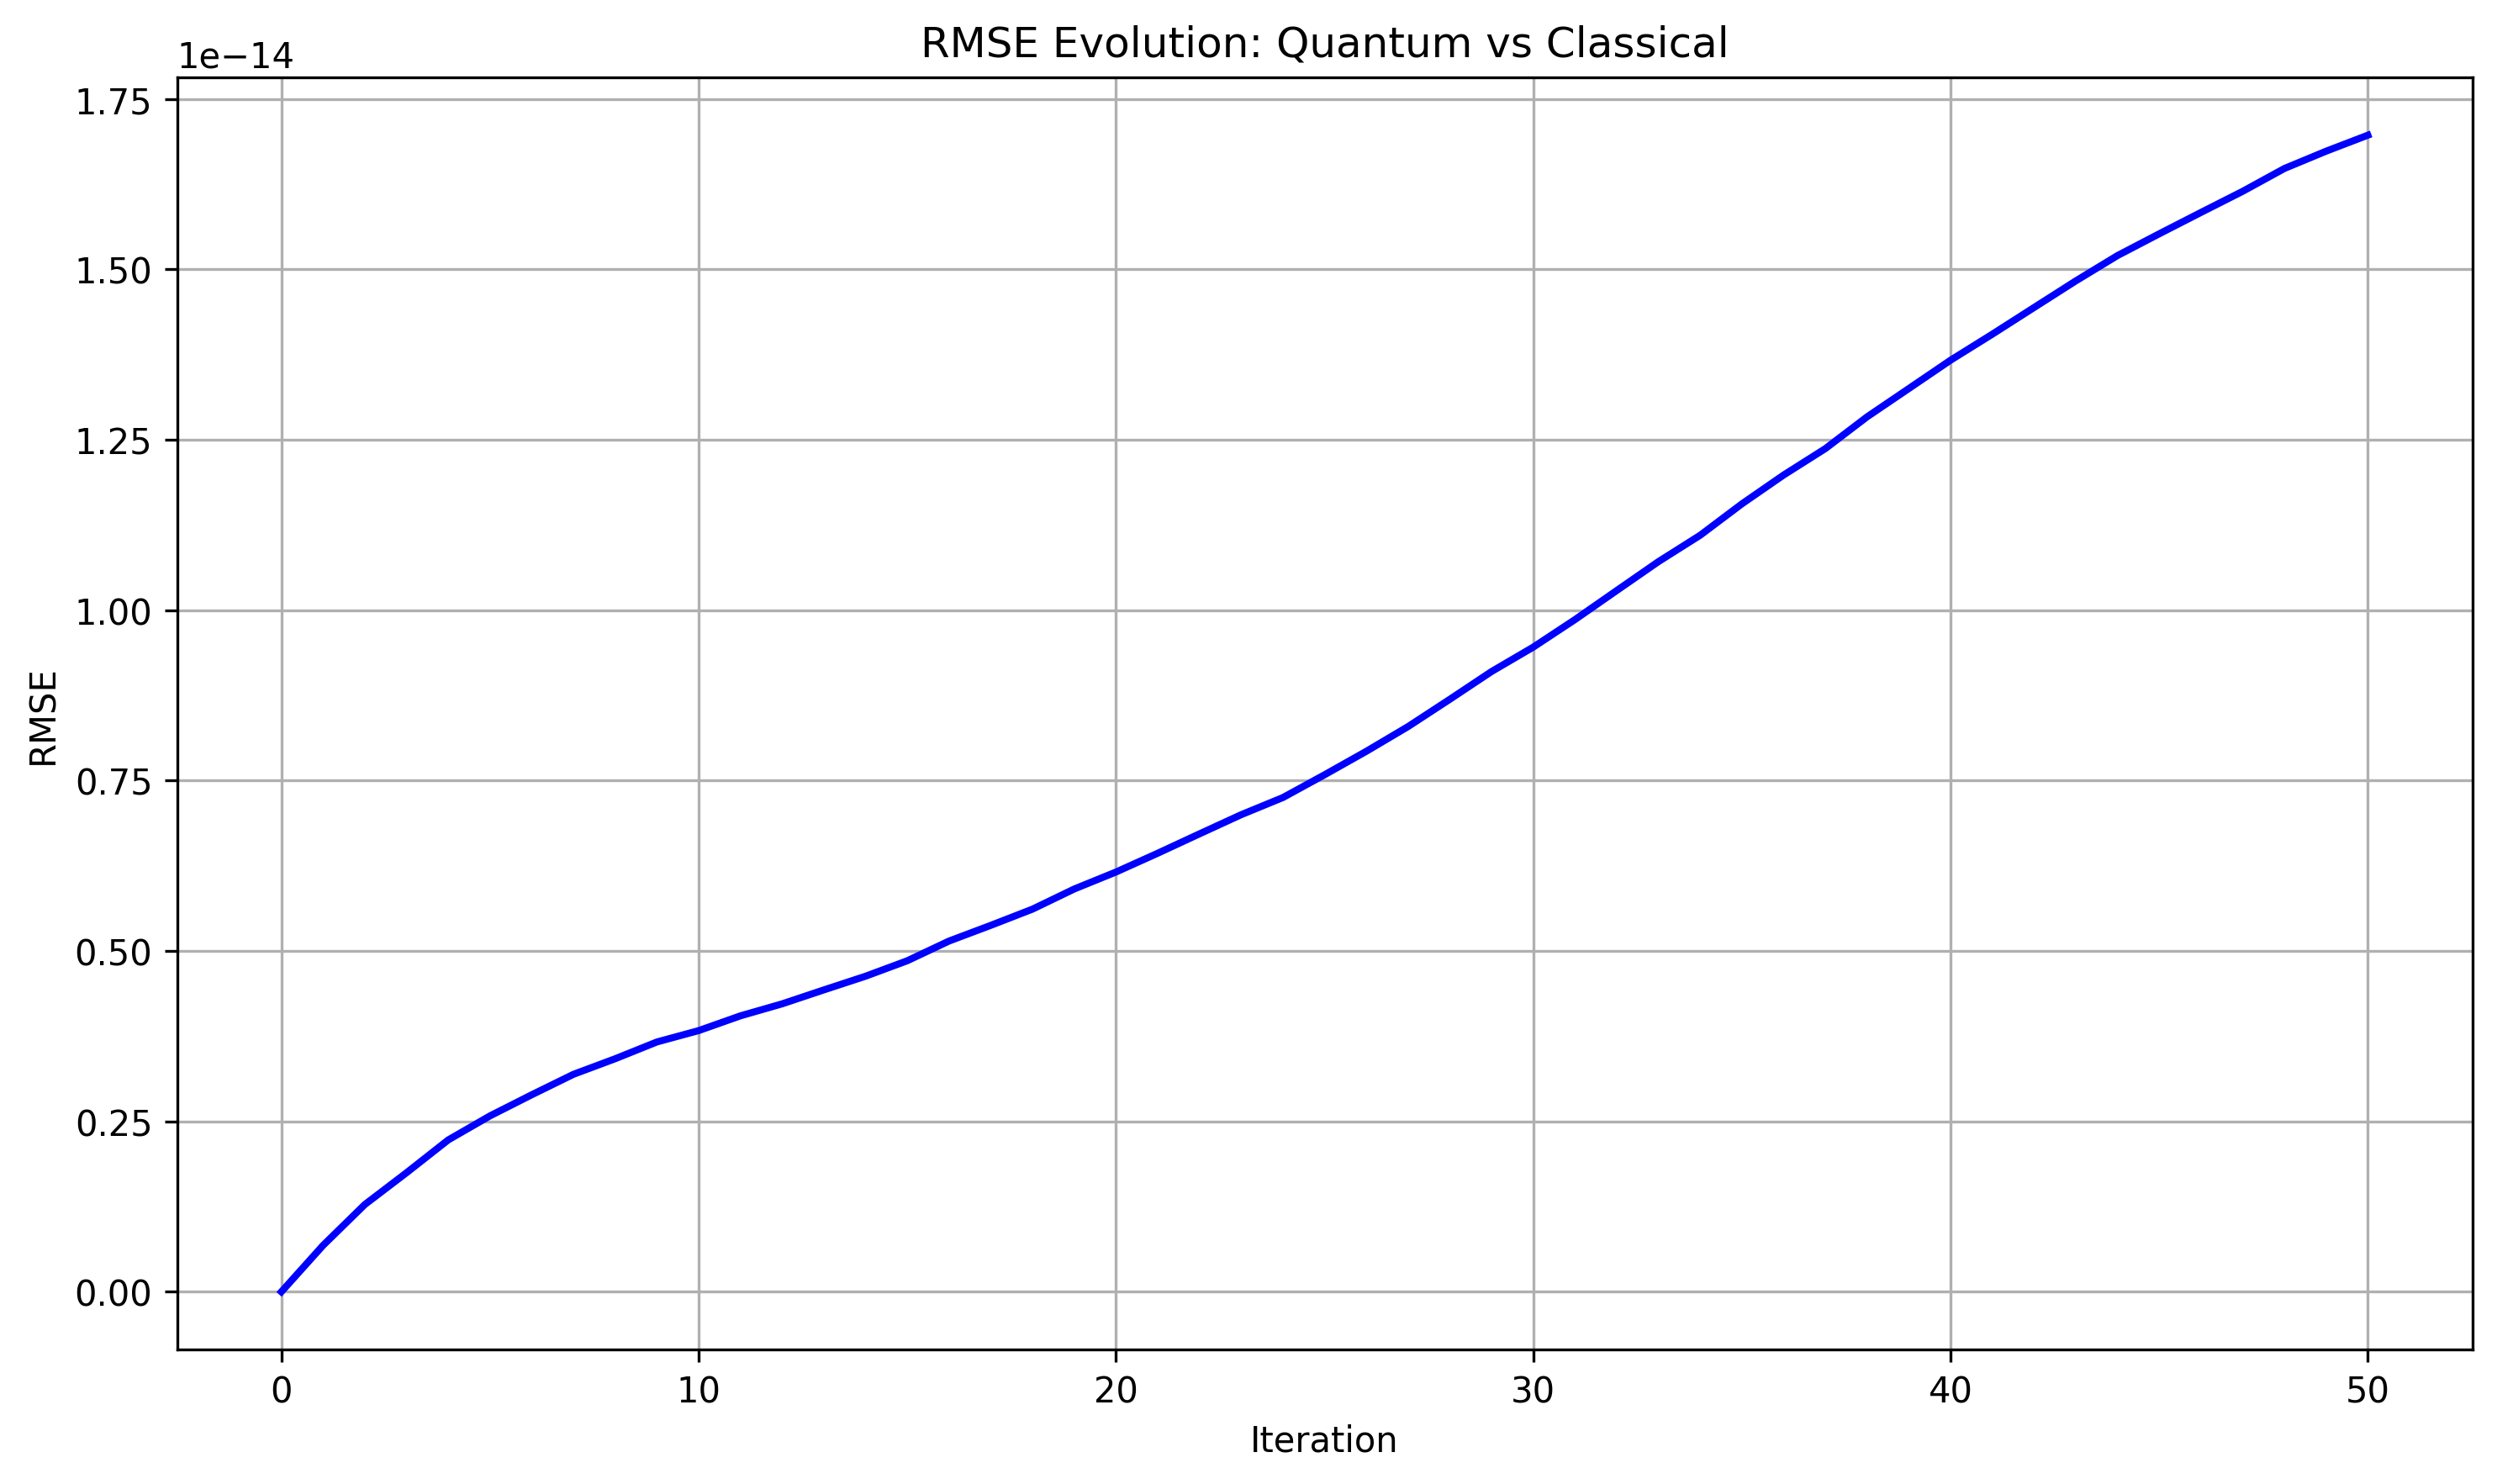
\includegraphics[width=0.7\textwidth]{src/img/figures/1_Drmse_plot.png}
    \caption{RMSE between classical and quantum for the 1D Gaussian experiment}
    \label{fig:rmse1d}
\end{figure}

\paragraph*{2D Simulation}
\begin{itemize}
    \item \textbf{Configuration:} D2Q9 with $32 \times 16$ lattice sites for 40 iterations.
    \item \textbf{Links:} $\{(0,0),(\pm1,0),(0,\pm1),(\pm1,\pm1)\}$ with weights $4/9$ (stationary), $1/9$ (orthogonal), $1/36$ (diagonal).
    \item \textbf{Initial condition:} Ring with outer radius $4$, inner radius $2$ of amplitude $0.9$ and background $0.1$.
    \item \textbf{Velocity field:} Shear field with $u=0.2$ in the bottom half, $u=-0.2$ in the top half, $v=0.1$ throughout.
\end{itemize}

\begin{figure}[H]
    \centering
    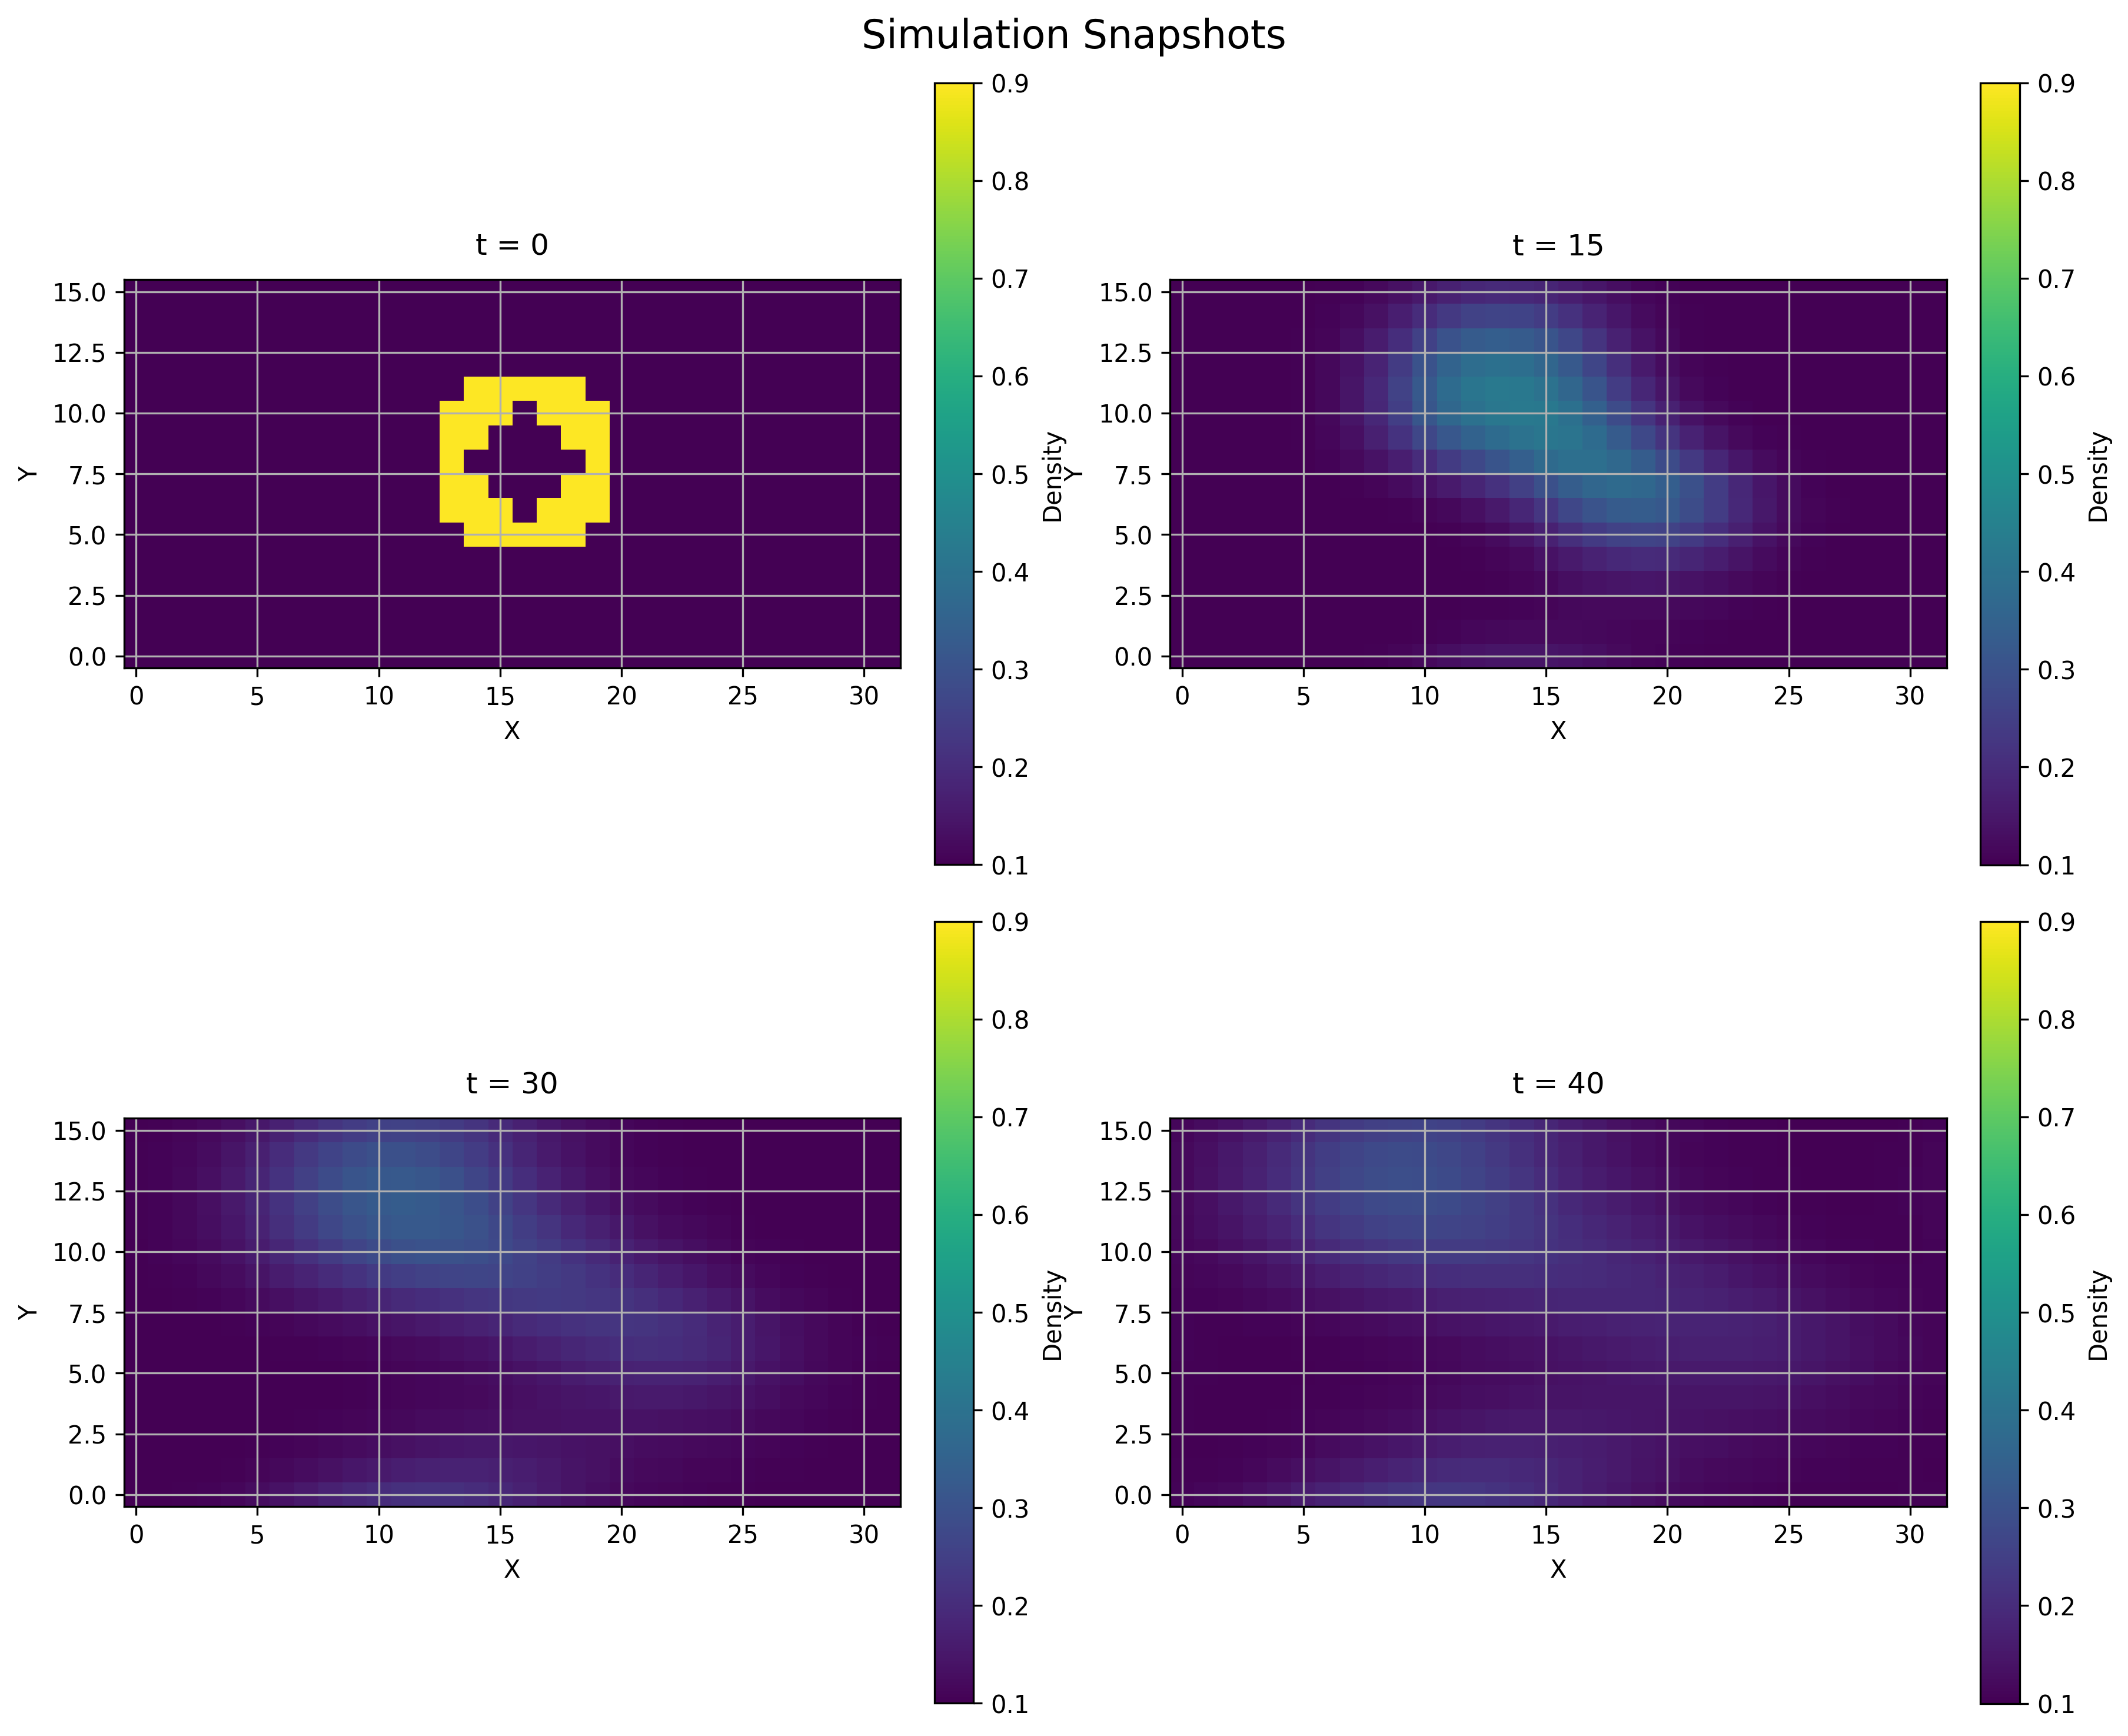
\includegraphics[width=\textwidth]{src/img/figures/2_Dquantum.png}
    \caption{Heatmap evolution of the 2D simulation with non-uniform velocity field}
    \label{fig:2d_snapshots}
\end{figure}

This experiment also shows an exact match, with an RMSE in the order of $10^{-14}$.

\begin{figure}[H]
    \centering
    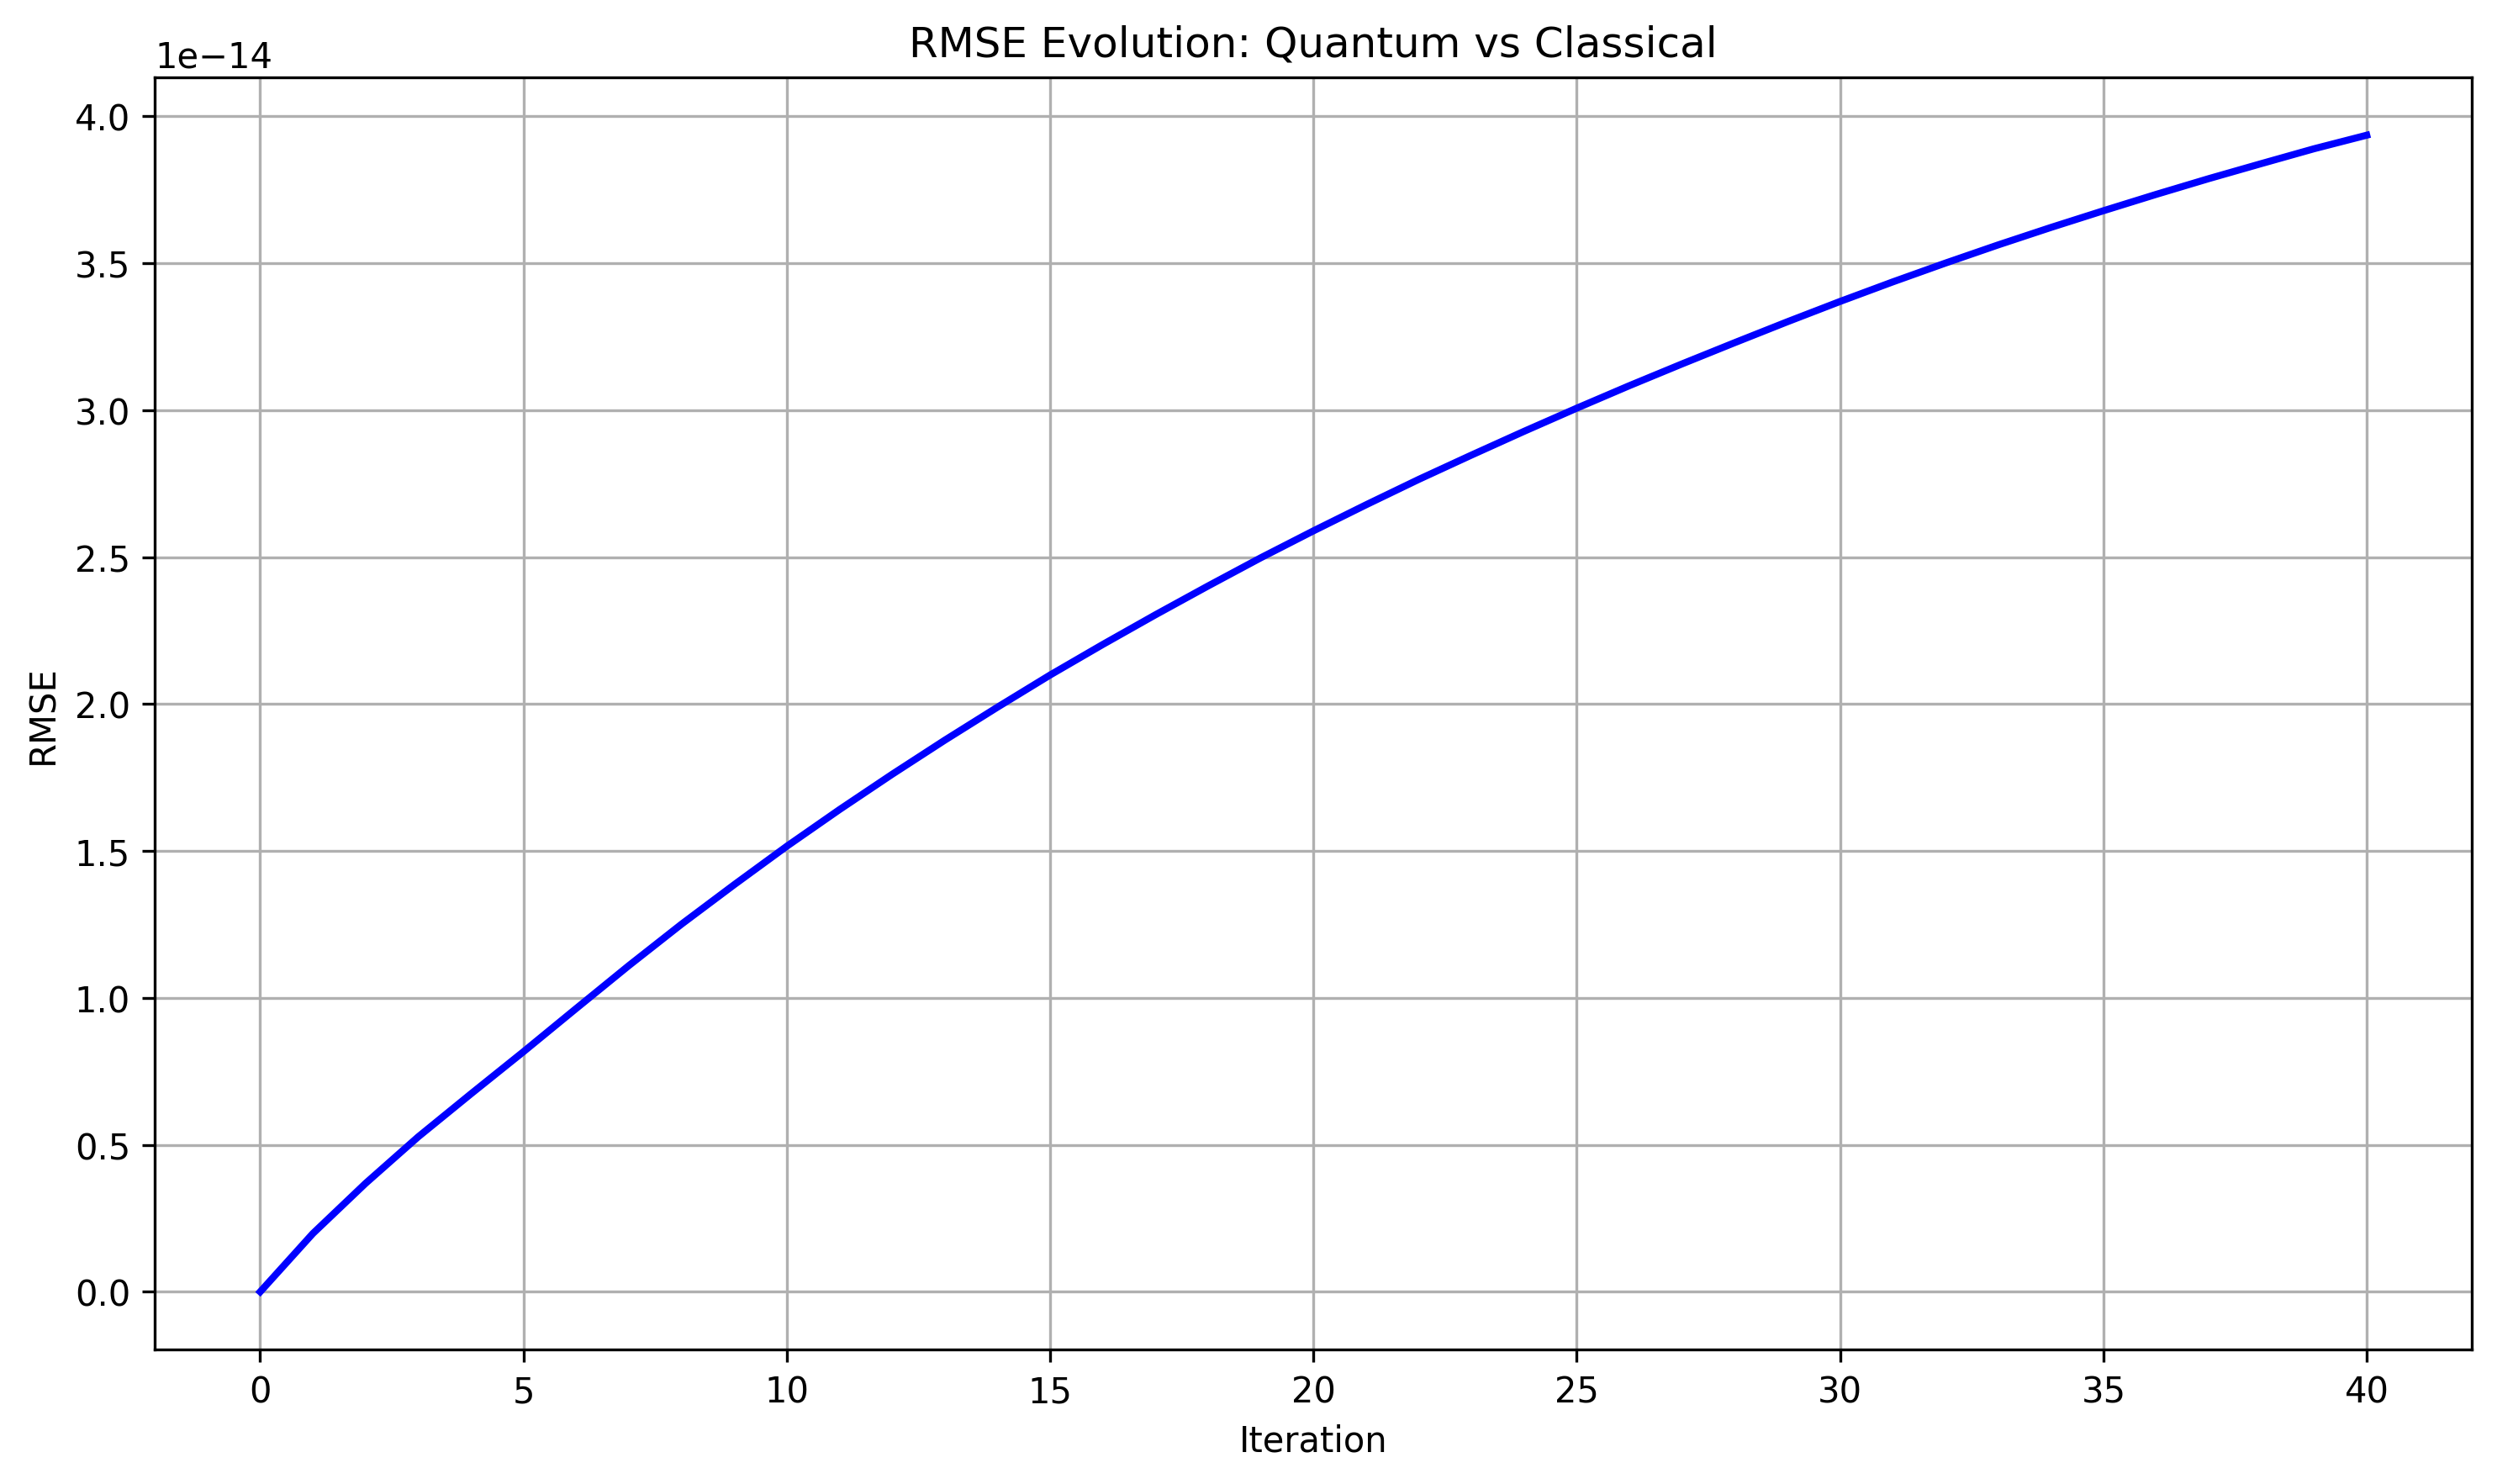
\includegraphics[width=0.9\textwidth]{src/img/figures/2_Drmse_plot.png}
    \caption{RMSE between classical and quantum for the 2D shear flow experiment}
    \label{fig:rmse2d}
\end{figure}

\paragraph*{3D Simulation}
\begin{itemize}
    \item \textbf{Configuration:} D3Q27 with $8 \times 8 \times 8$ lattice sites for 10 iterations.
    \item \textbf{Links:} Rest link, 6 orthogonal, 12 edge, 8 corner neighbors, with weights $8/27$, $2/27$, $1/54$, $1/216$ respectively.
    \item \textbf{Initial condition:} Three perpendicular planes through the grid center with density $0.9$ on planes and background $0.1$.
    \item \textbf{Velocity field:} Given by the following equations with amplitudes $A=B=C=0.2$ and spatial frequencies $a=b=c=1.0$:
    \begin{align*}
        u &= A\cos(ax)\sin(by)\sin(cz), \quad
        v  = B\sin(ax)\cos(by)\sin(cz), \quad
        w  = C\sin(ax)\sin(by)\cos(cz)
    \end{align*}
\end{itemize}

This is the parametrization for a Taylor-Green Vortex, a classic benchmark for LBMs.

\begin{figure}[H]
    \centering
    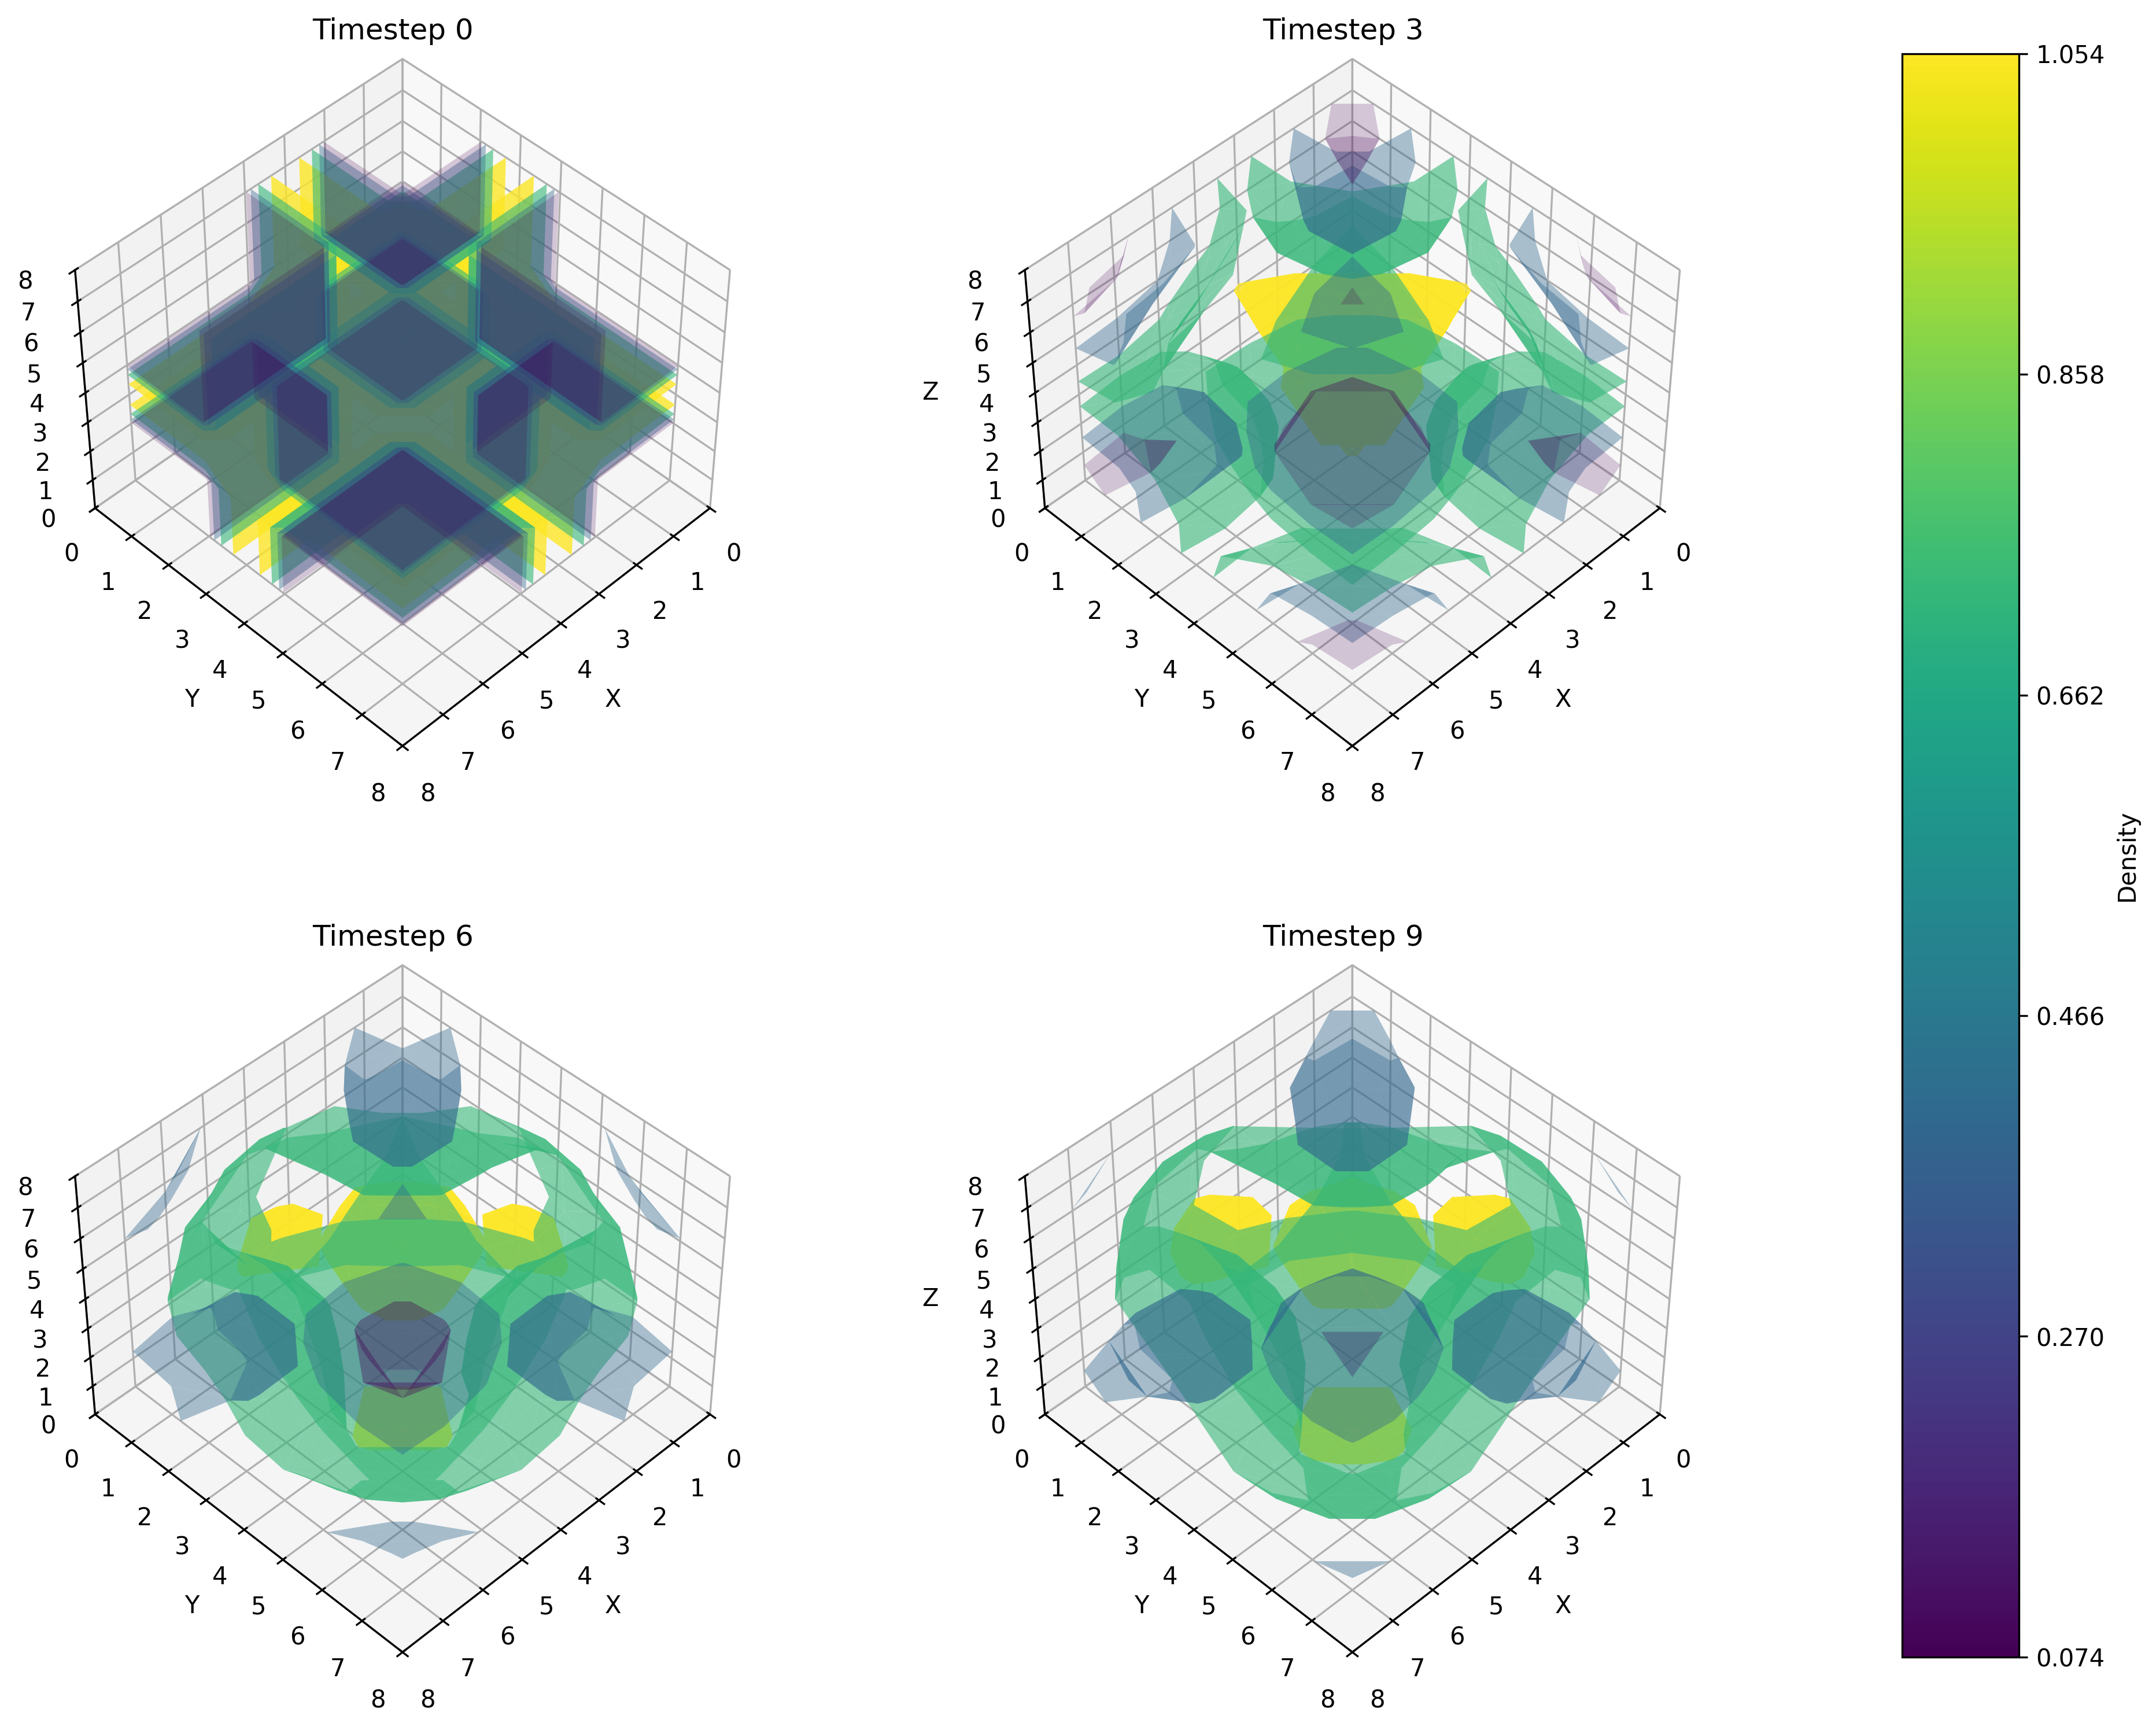
\includegraphics[width=\textwidth]{src/img/figures/3_Dquantum_snapshots.png}
    \caption{Isosurface evolution of the 3D simulation with non-uniform velocity field}
    \label{fig:3d_snapshots}
\end{figure}

This configuration yielded the highest error out of all the experiments at around $10^{-4}$
I do not yet have a concrete explanation for it, but the current hypothesis is the complex velocity field.

\begin{figure}[H]
    \centering
    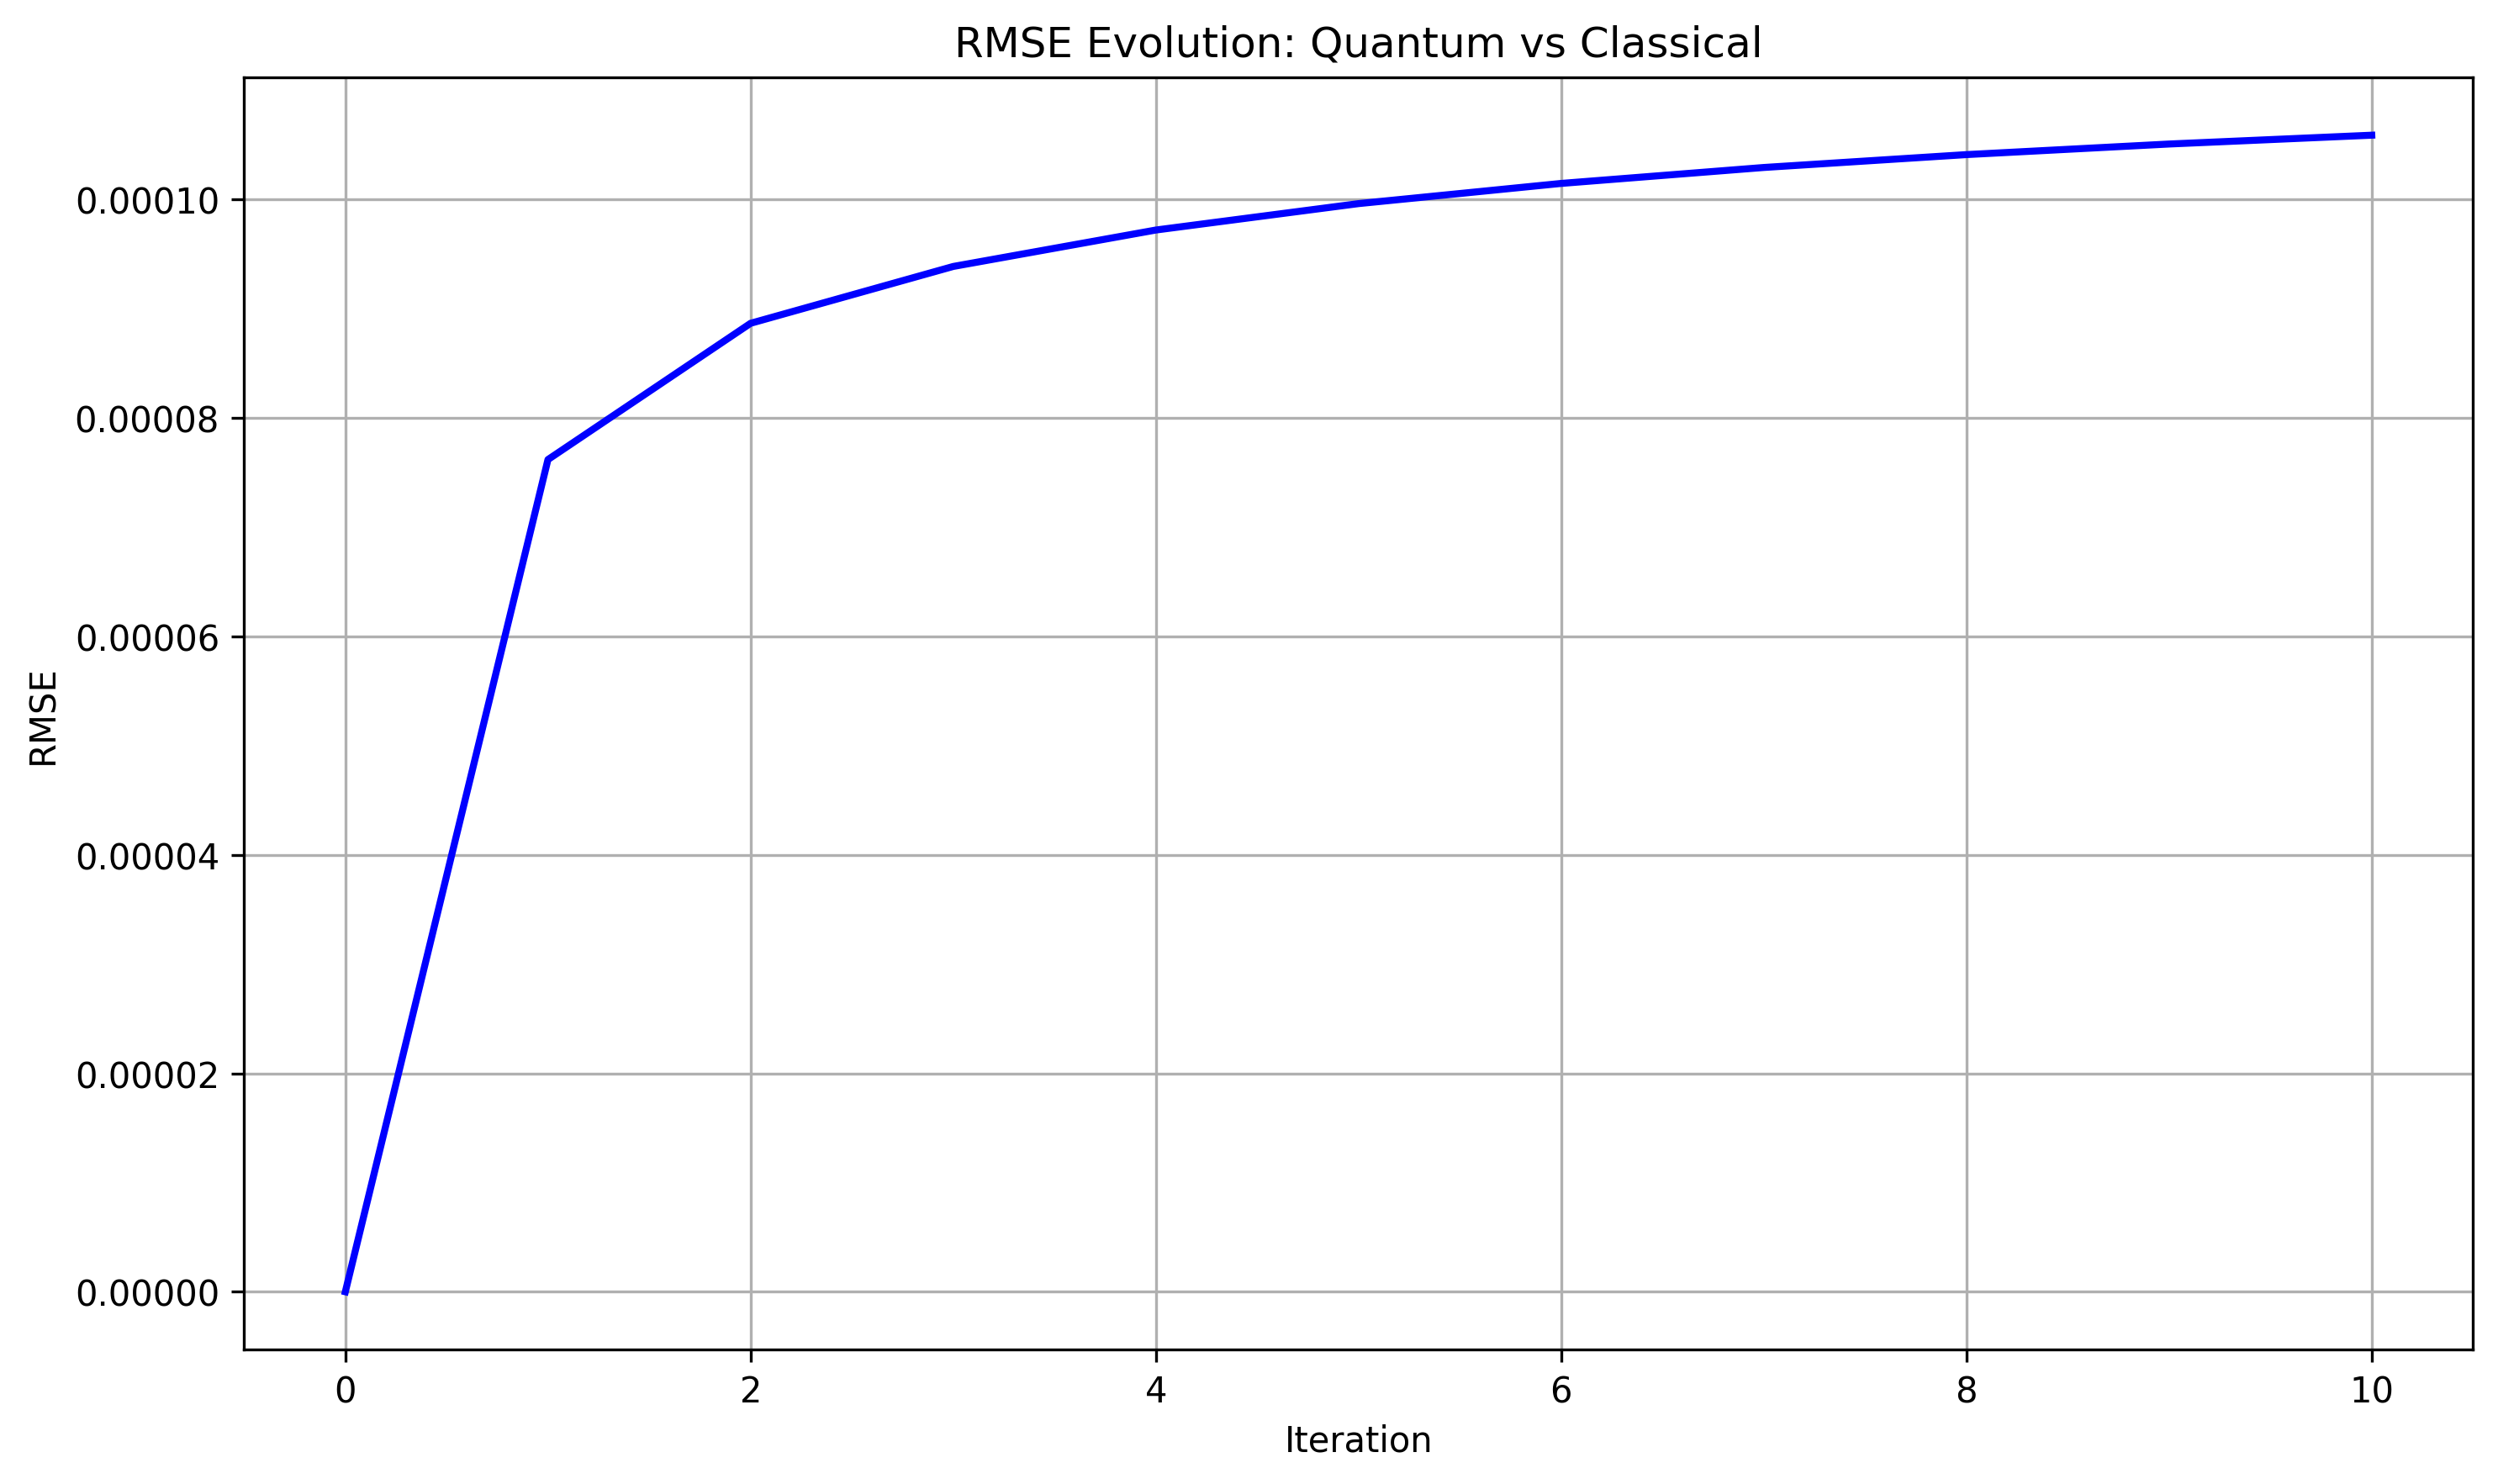
\includegraphics[width=0.8\textwidth]{src/img/figures/3_Drmse_plot.png}
    \caption{RMSE between classical and quantum for the 3D Taylor-Green vortex experiment}
    \label{fig:rmse3d}
\end{figure}

\paragraph*{2D Simulation with Non-Standard Link Velocities}
\begin{itemize}
    \item \textbf{Configuration:} $32 \times 32$ lattice sites for 25 iterations over two phases.
    \item \textbf{Initial condition:} Cross shape 4 cells wide with density $0.9$ and background $0.1$.
    \item \textbf{Phase 1 (15 iterations):} D2Q9 links with weights $\{4/9, 1/9, 1/36\}$; clockwise rotation vortex of magnitude $u=0.5$.
    \item \textbf{Phase 2 (10 iterations):} Non-standard links $\{(0,0),(2,1),(-2,-1)\}$ with weights $\{2/3,1/6,1/6\}$; zero velocity field.
\end{itemize}

You may notice that the the final 10 iterations have parameters that no longer recover the ADE.
Indeed this experiment no longer models the usual phenomena for which the equation was designed, but this does not make it worthless.
Other than serving as a numerical stress test, such a configuration can be used to simulate materials in which transport properties are not uniform across all directions.
This behavior is called \emph{anisotropic transport}.

\begin{figure}[H]
    \centering
    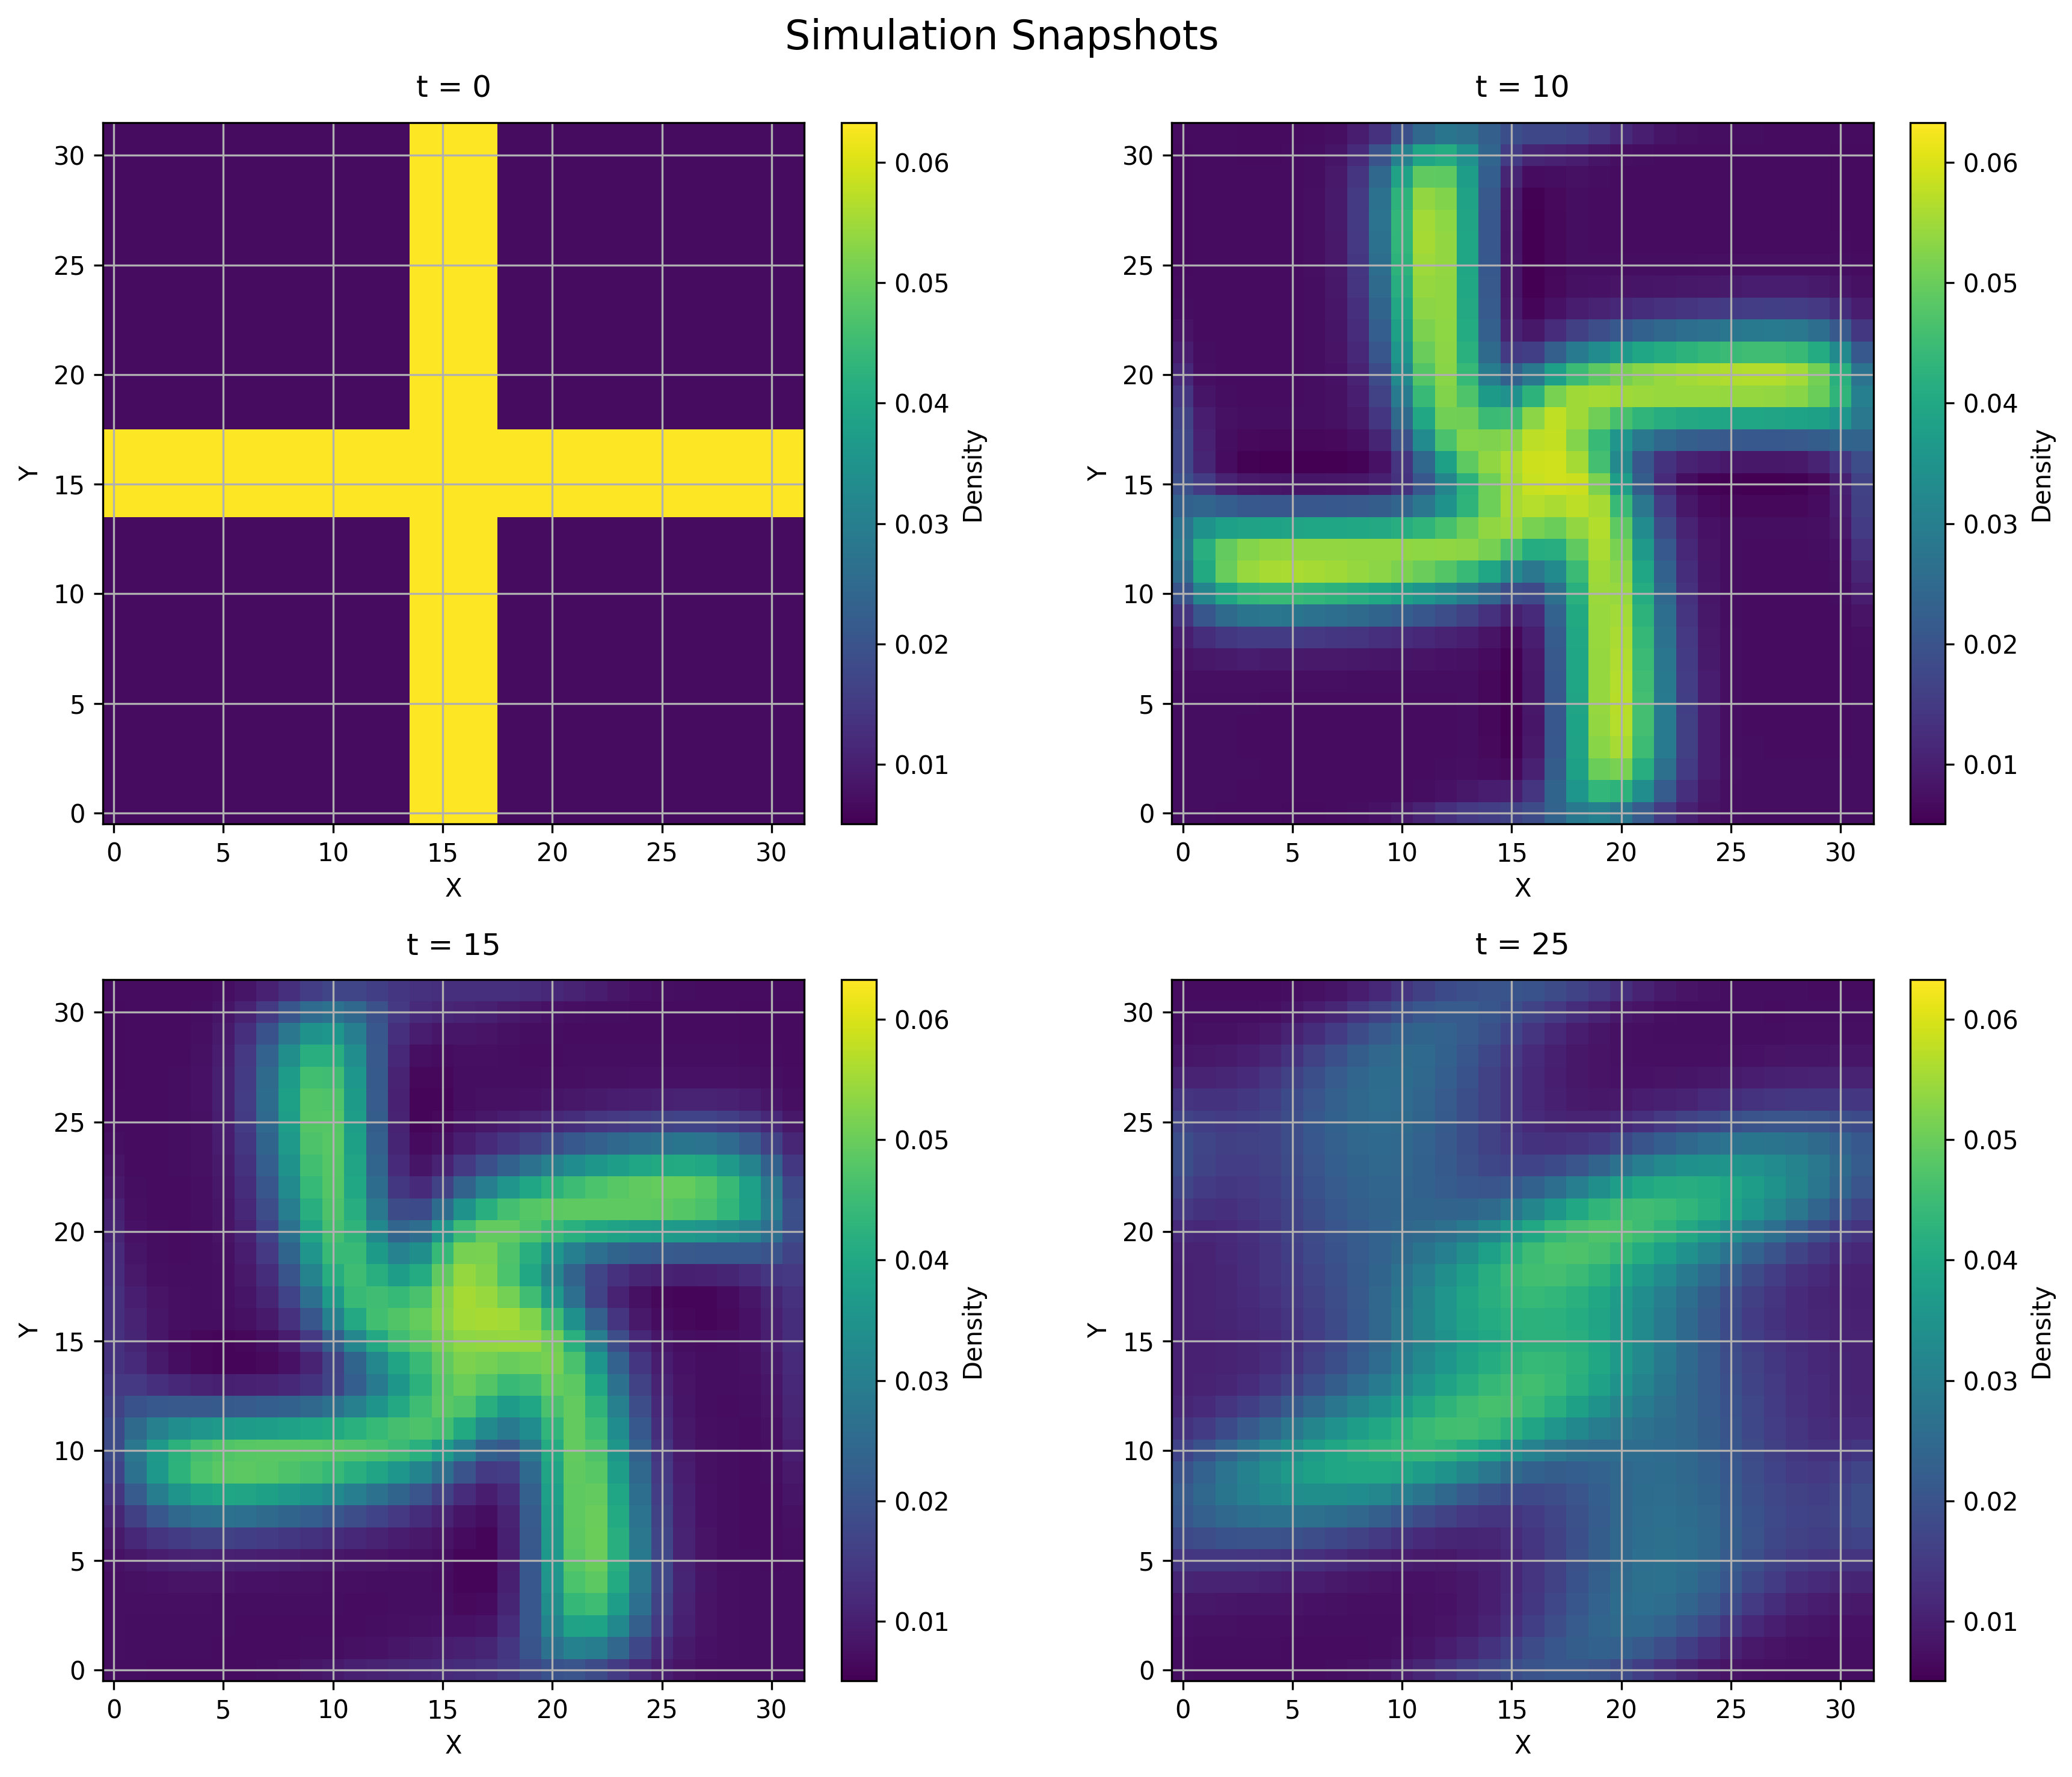
\includegraphics[width=0.9\textwidth]{src/img/figures/cross_quantum_snapshots.png}
    \caption{Heatmap evolution of the 2D simulation with time-varying velocity field and non-standard link velocities}
    \label{fig:cross_snapshots}
\end{figure}

Another relatively high error compared to the simple scenarios. Interestingly, the RMSE starts decreasing once the velocity field is removed.
This leads credence to the hypothesis for complex velocity fields.

\begin{figure}[H]
    \centering
    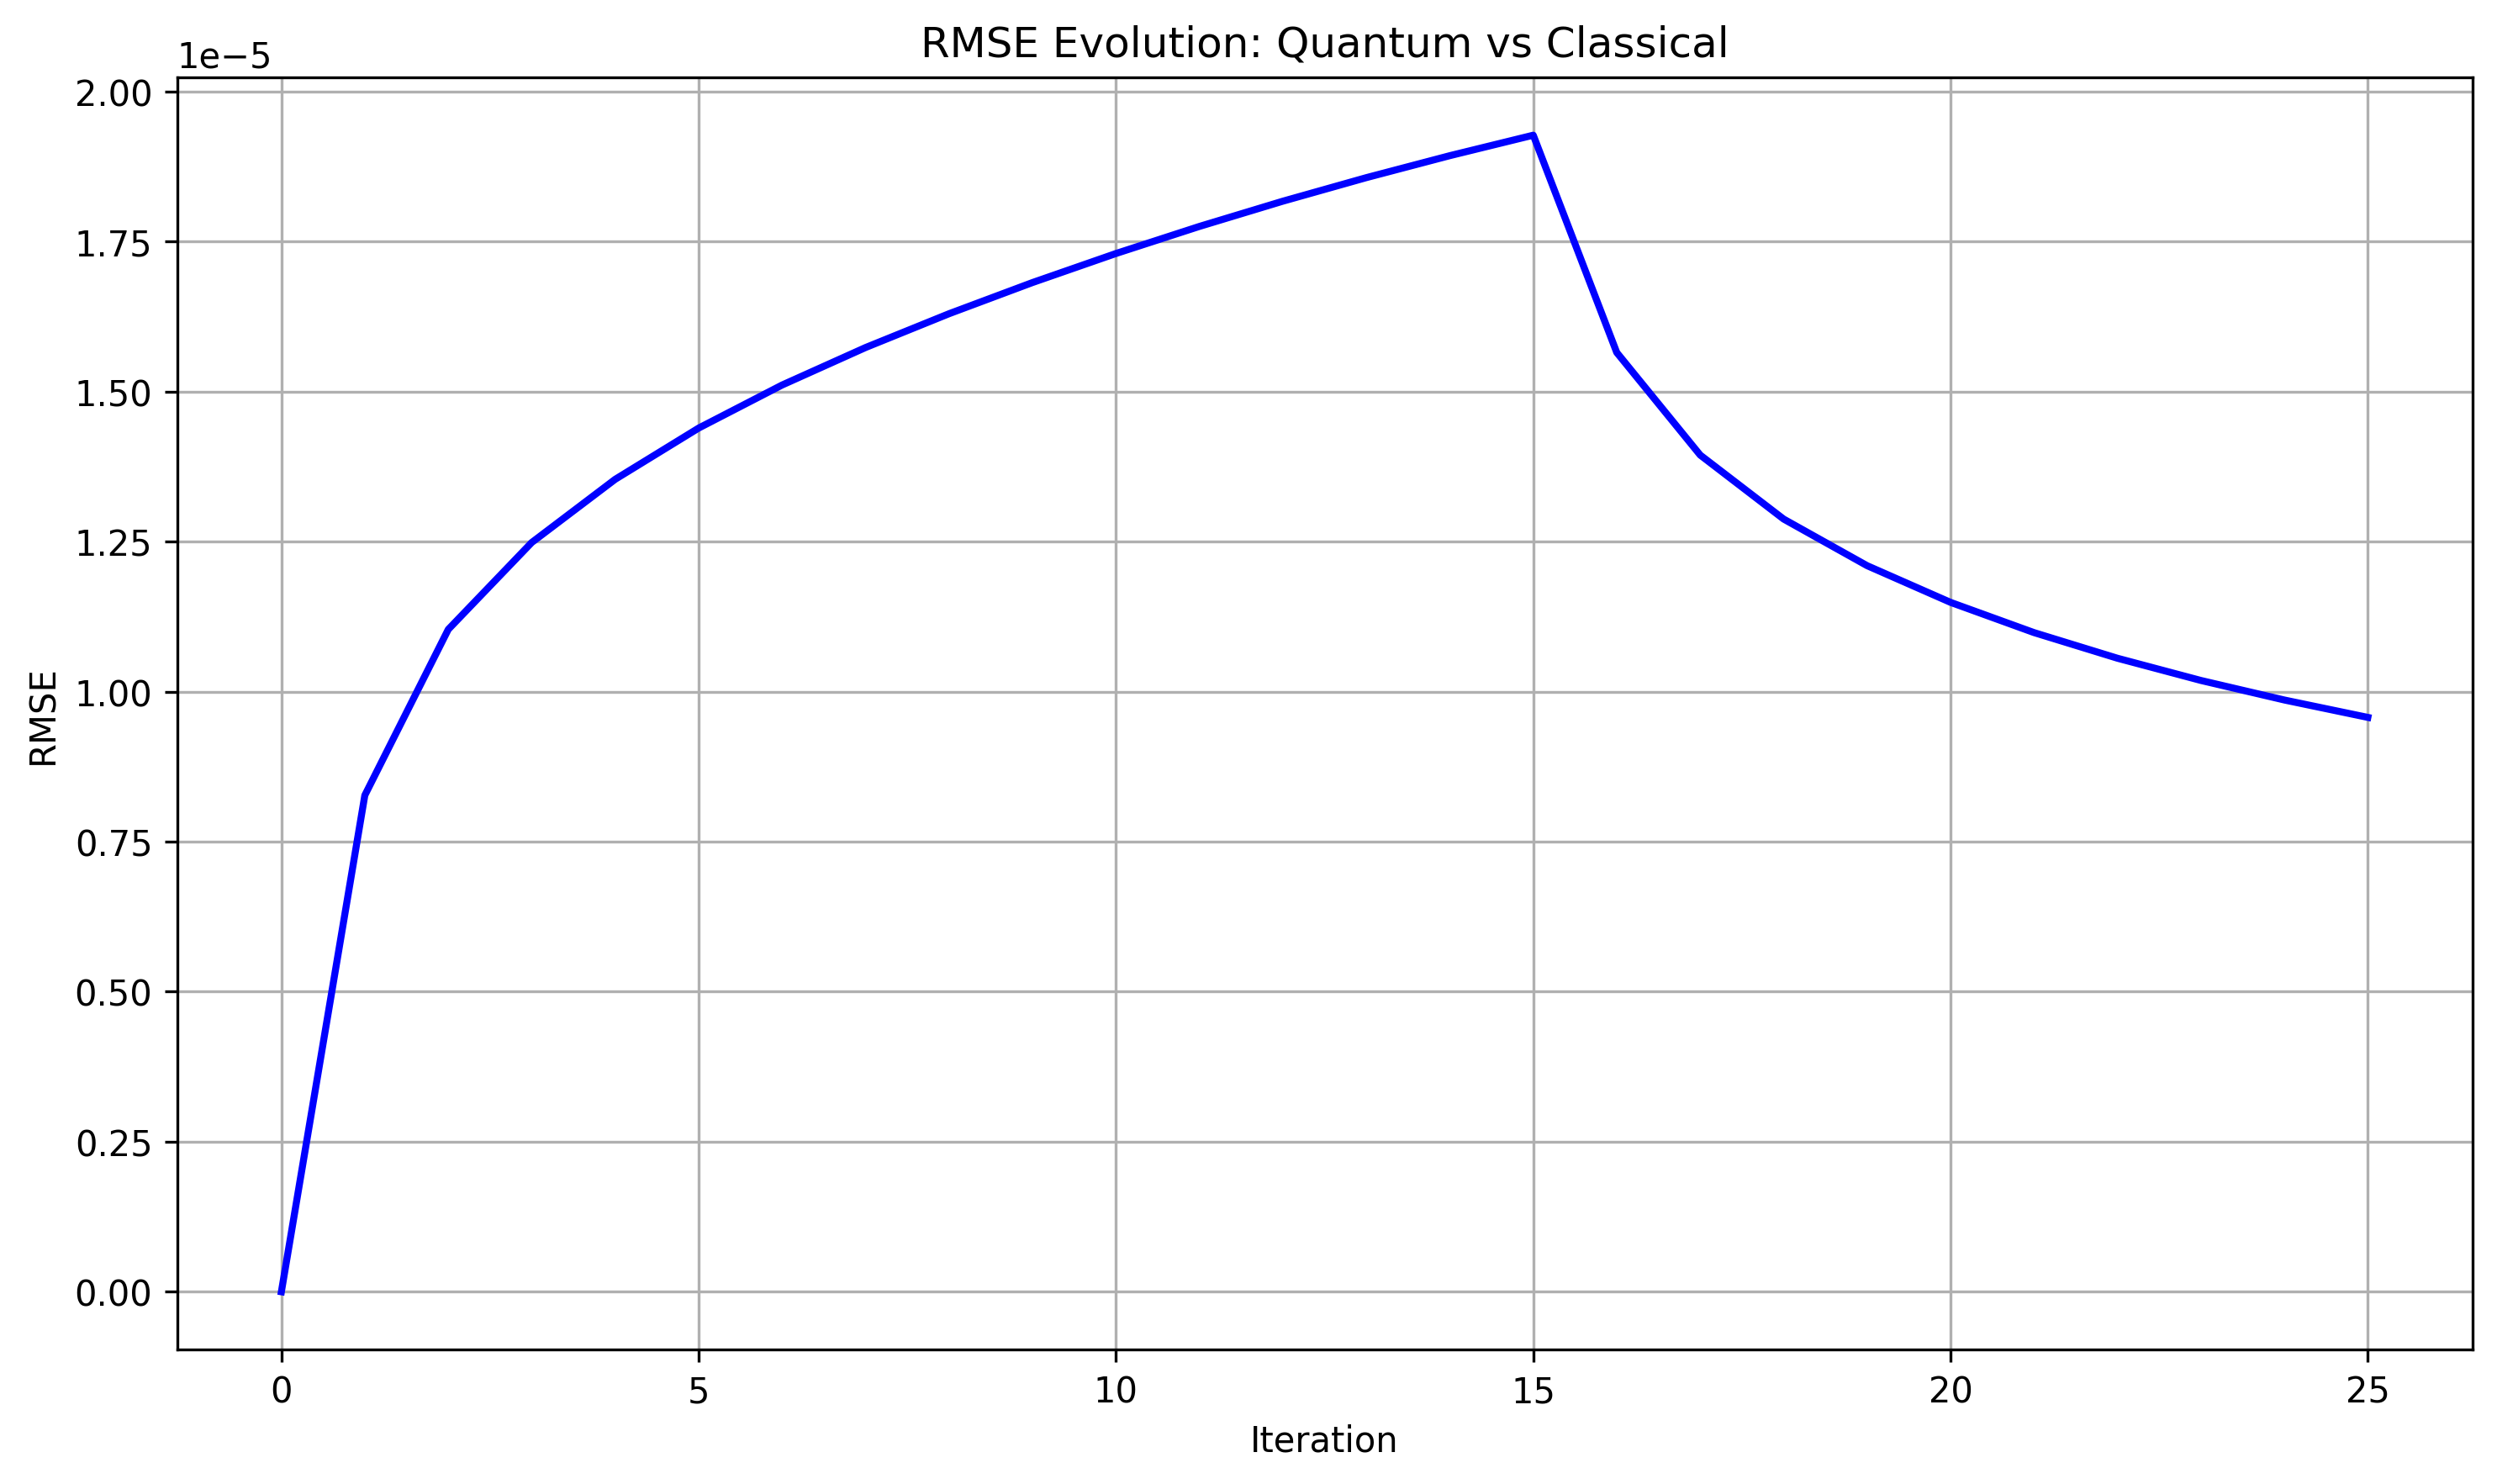
\includegraphics[width=0.7\textwidth]{src/img/figures/cross_rmse_plot.png}
    \caption{RMSE between classical and quantum for the 2D non-standard link velocity experiment}
    \label{fig:rmsecross}
\end{figure}

\section{Complexity Analysis}
\label{sec:complexity}

For a classical LBM simulating the ADE, both the time and space complexities are linear in the total number of lattice sites and link directions.
Given a lattice with a total of $M=\sum_{i=0}^{d}M_i$ sites and $N$ propagation directions, the complexity is $\mathcal{O}(M\cdot N)$ \cite{kruger2016lattice}.
This is complexity does not depend on the specifics such as the velocity field.

For my QLBM I already established in the previous section that the total number of qubits used is $n+m+1$. Writing the sum in terms of $M$ and $N$ results in a logarithmic complexity: $\mathcal{O}(\log{M} + log{N})$.
Since I am encoding information in superposition states, it's natural to see an improvement here.

Analyzing the time complexity is not so straightforward.
First of all, in a quantum circuit we are usually interested in the \emph{circuit depth}: the number sequential of quantum gates used to implement the circuit as a function of the size of the input.
When counting this depth, gates applied "in parallel" on different qubits can be considered constant time.
In addition, we only count elementary gates, ie: the aforementioned \texttt{DiagonalGate} is not constant time, but a perhaps exponential depending on the gate decomposition.
Which gates are elementary usually depends on the physical implementation of the quantum computer used.

\paragraph*{Initialization} is performed entirely by the Qiskit \texttt{initialize} function.
Internally, it makes use of Iten et al.'s exponential procedure \cite{iten2016isometries}.
Since I only initialize the $m$ lattice qubits, this results in a time complexity of $\mathcal{O}(2^m)$ or $\mathcal{O}(M)$.
The following $H$ gates applied on the velocity qubits, which is $\mathcal{O}(1)$.
All in all, the initialization step is linear.

\paragraph*{Collision} is defined as a linear combination of unitaries, with each unitary gate being a diagonal.
Naturally the bottleneck of this stage will be the decomposition of the diagonal gates into elementary ones.
The procedure used by Qiskit's \texttt{DiagonalGate} is based on Malvetti's work \cite{malvetti2018synthesis}. The decomposition's depth is exponential in the matrix's dimension.
Since I am manually computing the controlled unitaries, each matrix is $n+m+1 \times n+m+1$, meaning the final worst case complexity for the collision stage is $\mathcal{O}(2^{(m+n)})$ or $\mathcal{O}(M\cdot N)$.
Note however that this is the worst case complexity, when the velocity field is chaotic.
With a highly structured velocity field, the diagonals end up much easier to decompose, achieving potential polynomial or even constant complexity.

\paragraph*{Streaming} is a direct improvement over the classical counterpart.
As per the circuits in Figures~\ref{fig:l_gate} and \ref{fig:r_gate}, each shifting circuit has a linear depth of exactly $\log{M_i}$.
For each link velocity vector, the number of times we apply each circuit depends on the velocity vector itself.
Let's denote the average number of circuits applied for link velocity with $q$.
The worst case complexity for the streaming step thus works out to $\mathcal{O}(N\cdot q\cdot\log{M})$.
That being said, this worst case is only achieved when $q$ itself is significant.
In the average case, $q \ll N$, usually between 1 and 2, so the average case complexity is $\mathcal{O}(N\cdot\log{M})$
Note however that this assumes arbitrary multi-controlled gates are elementary, which is a fairly strong assumption.

\paragraph*{Macros computation} is linear with respect to number of links: $\mathcal{O}(N)$; as previously described.

Since all of these steps steps are in sequence, the total complexity is dominated by either the initialization or the collision step.
The actual details will depend heavily on the particular simulation parameters chosen, mostly the velocity field.

\subsection{Numerical Benchmarks}

In addition to the theoretical analysis, I have performed a concrete numerical analysis for the gate count and circuit depth of each stage under various configurations.
The chosen elementary gate set was the IBM Eagle native set: $\{R_z, \sqrt{X}, X, \text{CX}\}$ \cite{ibm_quantum_2026}.

The data in Table~\ref{tab:transpilation} supports the theoretical analysis.

The biggest and most surprising observation is that gate counts are generally higher than expected.
Even accounting for exponential complexity in the number of qubits, the measured values can only be explained by large constants.   

The collision is the clear bottleneck. 
As expected, the complexity of the velocity field is directly proportional to the circuit depth.
Otherwise it follows the expected trend as the qubit count grows.

The streaming step also shows a surprisingly high circuit depth compared to the analytical result.
In reality it is not so surprising considering that the multi-controlled gates used are not elementary.
Another comtributing factor is that at low $N$ and $M$ values, constants dominate the complexity.
This is supported by the observation that despite starting fairly equally, collision overtakes streaming in larger simulations.
Lastly, the final depth is mostly influenced by lattice sites per dimension: the 4x4x4 3D simulation results in a smaller circuit compared to the 8x8 2D ones, despite identical $M$.

\begin{table}[H]
\centering
\caption{Transpiled gate count and circuit depth (gates / depth) per stage}
\label{tab:transpilation}
\resizebox{\textwidth}{!}{%
\begin{tabular}{l c r r r r r r}
\toprule
Configuration & Qubits & Initialize & Encode Links & Collision & Streaming & Macros & \textbf{Total} \\
\midrule
D1Q3 $M{=}4$ & 5 & 86 / 81 & 6 / 3 & 393 / 270 & 101 / 69 & 6 / 3 & \textbf{592 / 426} \\
D1Q3 $M{=}8$ & 6 & 129 / 118 & 6 / 3 & 786 / 540 & 663 / 491 & 6 / 3 & \textbf{1,590 / 1,155} \\
D1Q3 $M{=}16$ & 7 & 172 / 155 & 6 / 3 & 1,563 / 1,066 & 1,947 / 1,453 & 6 / 3 & \textbf{3,694 / 2,680} \\
\midrule
D1Q3 $M{=}16$ uniform $v$ & 7 & 172 / 155 & 6 / 3 & 1,563 / 1,066 & 1,947 / 1,453 & 6 / 3 & \textbf{3,694 / 2,680} \\
D1Q3 $M{=}16$ gradient $v$ & 7 & 172 / 155 & 6 / 3 & 2,135 / 1,581 & 1,947 / 1,453 & 6 / 3 & \textbf{4,266 / 3,195} \\
D1Q3 $M{=}16$ zero $v$ & 7 & 172 / 155 & 6 / 3 & 1,567 / 1,070 & 1,947 / 1,453 & 6 / 3 & \textbf{3,698 / 2,684} \\
\midrule
D2Q9 $8{\times}8$ shear & 11 & 1,122 / 1,093 & 12 / 3 & 24,991 / 16,785 & 14,890 / 11,660 & 12 / 3 & \textbf{41,027 / 29,544} \\
D2Q9 $8{\times}8$ vortex & 11 & 1,122 / 1,093 & 12 / 3 & 38,739 / 30,453 & 14,890 / 11,660 & 12 / 3 & \textbf{54,775 / 43,212} \\
D2 nonstandard $8{\times}8$ & 9 & 258 / 229 & 6 / 3 & 6,194 / 4,170 & 1,935 / 1,449 & 6 / 3 & \textbf{8,399 / 5,854} \\
\midrule
D3Q27 $4{\times}4{\times}4$ & 12 & 2,274 / 2,245 & 15 / 3 & 59,457 / 43,060 & 4,695 / 3,805 & 15 / 3 & \textbf{66,456 / 49,116} \\
\bottomrule
\end{tabular}%
}
\end{table}

Unlike the other stages which can be transpiled once per configuration and cached, initialization must be redone each iteration since
it directly depends on the distribution.
In Table~\ref{tab:init_per_iter} I counted the total gates and circuit depth for each iteration as the distribution evolves for a given configuration.
Notice how the first iteration has a noticeable lower circuit depth, this is due to the extra structure of the initial distribution (a gaussian ring).
As the simulation evolves and distribution becomes more chaotic, the depth increases but quickly stabilizes.

\begin{table}[H]
\centering
\caption{Per-iteration initialization gate count for D2Q9 $8{\times}8$ shear flow}
\label{tab:init_per_iter}
\begin{tabular}{c r r}
\toprule
Iteration & Init.\ Gates & Total Gates \\
\midrule
1 & 8,449 & 48,354 \\
2 & 10,402 & 50,307 \\
3 & 10,440 & 50,345 \\
4 & 10,346 & 50,251 \\
5 & 10,575 & 50,480 \\
6 & 10,560 & 50,465 \\
7 & 10,337 & 50,242 \\
8 & 10,354 & 50,259 \\
9 & 10,240 & 50,145 \\
\bottomrule
\end{tabular}
\end{table}

\section{}